\begin{apendicesenv}

\partapendices

\chapter{Termo de Abertura do Projeto}
	\label{tap}
% 	\input{anexos/Termo_de_abertura}

%%%%%%%%%%%%%%%%%%%%%%%% INICIO DO TAP
\begin{center}
 {\large Termo de abertura}\\[0.2cm]
 {Bancada para Ensaios de Vibração Mecânica}\\
 \end{center}
 
 \section*{Histórico de Alterações}
\begin{table}[h]
\centering
\begin{tabular}{|c|c|p{6cm}|p{5cm}|}
\hline
Data & Versão & Descrição & Responsável\\
\hline                               
26/08/2016 & 1.0 & Criação do documento. & Anderson Tenório, Ítalo Paiva e Paulo Borba .\\
\hline                               
27/08/2016 & 1.1 & Reformulação da estrutura do documento. & Ítalo Paiva.\\
\hline
\end{tabular}
\end{table}

\section*{Nome do projeto}
  Bancada para Ensaios de Vibração Mecânica.
  
\section*{Descrição do projeto}

    O projeto visa desenvolver uma bancada para ensaios de vibração mecânica
    genérica para os alunos dos cursos de Engenharia Automotiva e Aeroespacial
    da UnB-FGA (Faculdade do Gama) possam realizar testes de diversas estruturas
    nas disciplinas que os fizerem necessários.

\section*{Objetivos do projeto}
  
    Este trabalho tem por objetivo geral propor o projeto e implementação
    de uma bancada para ensaios de vibração mecânica para suprir a carência
    deste equipamento na UnB-FGA, que possui uma aplicação mais didática
    que industrial.

   São objetivos específicos do projeto:
   \begin{itemize}
    \item Elaborar o projeto mecânico/estrutural da bancada;
    \item Elaborar o projeto eletromecânico de funcionamento da bancada;
    \item Elaborar o projeto eletroeletrônico de funcionamento da bancada;
    \item Elaborar o projeto do sistema de monitoramento e controle da bancada;
    \item Integrar as soluções de cada frente de trabalho.
   \end{itemize}
  
\section*{Justificativa do projeto}
	
    %%%%%%%%%%%%%% Melhorar isso aqui
    
    A Faculdade UnB Gama conta com excelentes profissionais e alunos, porém 
    a falta de equipamentos especializados e infraestrutura para que os alunos 
    possam aprender melhor, é um problema antigo. Alguns equipamentos
    necessários para realização de testes faltam no \textit{campus}, o que
    acaba impactando negativamente a formação dos alunos de Engenharia
    Automotiva e Aeroespacial, principalmente.
    
    Com isso em mente, este projeto foi proposto para suprir a falta de
    um equipamento de testes de vibração na faculdade, área bastante explorada
    em disciplinas dos cursos de Engenharia Automotiva e Aeroespacial.
    
    %%%%%%%%%%%%%% Melhorar isso aqui

\section*{Recursos do produto}
	
    A solução apresentada conta com os seguintes recursos:
    
    \begin{itemize}
        \item Frequência controlada pelo usuário;
    	\item Calibração automática da frequência da mesa;
        \item Sensoreamento livre em dois locais de escolha do usuário;
        \item Aplicação \textit{web} para controle da bancada e visualização
        	  dos resultados.
    \end{itemize}
    
    \subsection*{Subprodutos identificados}
    
    	O projeto como um todo gerará os seguintes subprodutos:
        
        \begin{itemize}
        	\item \textbf{Estrutura física da bancada vibracional} - Projeto e produto
            			  da estrutura de sustentação, do mecanismo vibracional e da
                          estrutura da bancada. A bancada vibracional engloba tanto a
                          mesa vibratória e sua sustentação quanto os 
                          sensores acoplados na mesa para controle da frequência e os
                          sensores livres para o usuário.
        	\item \textbf{Sistema de Monitoramento e Controle da Bancada} - 
                          Aplicação \textit{web} responsável por controlar o
                          funcionamento da bancada, onde o usuário entrará com
                          os dados de entrada para o teste e visualizará os
                          resultados do teste. Além da aplicação, será fornecida
                          também toda a documentação associada.
        \end{itemize}

\section*{\textit{Stakeholders}}

Os envolvidos no projeto seja no desenvolvimento, na aquisição ou no uso da aplicação final são \textit{stakeholders}. Foram considerados envolvidos no projeto todos que tenham algum tipo de interesse e/ou participação, e a Tabela \ref{stakeholders_projeto} lista os \textit{stakeholders} identificados.
        
        \begin{table}[h]
            \centering
            \caption{Envolvidos no projeto}
            \label{stakeholders_projeto}
            \begin{tabular}{|c|c|c|}
            \hline
            \textbf{Nome}      & \textbf{Descrição}                                                                            & \textbf{Responsabilidades}                                                                                                              \\ \hline
            Integrantes do grupo & \begin{tabular}[c]{@{}c@{}}Integrantes do grupo de\\  desenvolvimento da bancada\end{tabular} & \begin{tabular}[c]{@{}c@{}}Acompanhar o desenvolvimento \\ e validar a integração do software\\  com os demais subprodutos\end{tabular} \\ \hline
            Professores de PI2 & Professor da disciplina de PI2                                                                & \begin{tabular}[c]{@{}c@{}}Monitorar o andamento do projeto; \\ Avaliar o projeto e o produto.\end{tabular}                             \\ \hline
            \begin{tabular}[c]{@{}c@{}}Alunos \\ (Automotiva e/ou \\ Aeroespacial)\end{tabular} & \begin{tabular}[c]{@{}c@{}}Usuário direto\\  do sistema\end{tabular} & \begin{tabular}[c]{@{}c@{}}Realizar testes no equipamento,\\  controlando a bancada.\end{tabular} \\ \hline
          Técnicos & \begin{tabular}[c]{@{}c@{}}Usuário direto \\ do sistema\end{tabular} & \begin{tabular}[c]{@{}c@{}}Gerenciar e acompanhar \\ o uso do equipamento.\end{tabular} \\ \hline
          \begin{tabular}[c]{@{}c@{}}Professores \\ (Automotiva e/ou \\ Aeroespacial)\end{tabular} & \begin{tabular}[c]{@{}c@{}}Usuário direto\\ do sistema\end{tabular} & \begin{tabular}[c]{@{}c@{}}Realizar testes no equipamento,\\  controlando a bancada\end{tabular} \\ \hline
            \end{tabular}
        \end{table}


\section*{Líderes do projeto e suas responsabilidades}

    Cada frente de trabalho possui uma interface de comunicação com o grupo todo.
    Esta interface é o líder da frente. 

    Então, o líder fica responsável por coordenar e dividir atividades entre a sua
    frente de trabalho e comunicar à equipe decisões, status de atividades e entre
    outras informações. Os líderes de cada frente, em conjunto com o grupo, são
    responsáveis por tomar decisões e representar o grupo como um todo.

    A relação dos líderes de cada frente de trabalho definida se encontra abaixo:

    \begin{itemize}
        \item \textbf{Frente Estrutural/Mecânica} - João Kaled
        \item \textbf{Frente Eletromecânica} - Anderson Andrade
        \item \textbf{Frente Eletroeletrônica} - Pedro Inazawa
        \item \textbf{Frente de Interface/Processamento} - Matheus Ferraz
    \end{itemize}

\section*{Cronograma de marcos sumarizado}

	A tabela abaixo apresenta os principais marcos do projeto em que serão responsáveis para realização
    de avaliações sobre o estado do projeto bem como entregas de protótipos funcionais e produto final,
    com as devidas datas de acordo com o cronograma.

  \begin{table}[h]
  \centering
  \begin{tabular}{|c|p{4.5cm}|p{8cm}|}
	\hline
  Data & Marcos & Descrição\\
  \hline                               
  19/08-06/08/2016 & Solução inicial & Definição da solução inicial do projeto a partir de ideias integradoras.\\
  \hline                               
  09/09/2016 & Ponto de Controle 1 & Apresentação da concepção do projeto com os requisitos bem definidos 
  									sobre o que será entregue e quais as características serão 												desenvolvidas para o produto a ser entregue.\\
  \hline                               
  12/09-03/11/2016 & Construção da solução & Desenvolvimento físico da bancada para ensaios de vibração mecânica.\\
  \hline                               
  09/11/2016 & Ponto de Controle 2 & Apresentação de um protótipo funcional e relatório do 
  									andamento do projeto.\\
  \hline                               
  26/10-30/11/2016 & Integração e Homologação & Integração das soluções e homologação da bancada para ensaios de vibração mecânica após realizados todos os testes.\\
  \hline
  02/12/2016 & Ponto de Controle 3 e Entrega Final do Produto & Apresentação do produto final, com os módulos 																	de cada engenharia integrados e que 																	estejam de acordo com os requisitos 																	elicitados inicialmente.\\
  \hline
  \end{tabular}
  \end{table}


\section*{Investimento preliminar}

	O custo total estimado do projeto é de R\$ 3.253,87.

\section*{Restrições e riscos}
	
    Os riscos identificados para o projeto estão listados na Tabela \ref{riscos_projeto_tap}, juntamente com a probabilidade, impacto e prioridade definidos (mais informações sobre os riscos do projeto podem ser obtidos no Plano de Gerenciamento de Riscos, no Apêndice \ref{plano_de_riscos}).

\begin{table}[h]
\centering
\caption{Riscos Identificados para o Projeto}
\label{riscos_projeto_tap}
\begin{tabular}{|l|l|l|c|}
\hline
\multicolumn{1}{|c|}{\textbf{Risco}} & \multicolumn{1}{c|}{\textbf{Probabilidade}} & \multicolumn{1}{c|}{\textbf{Impacto}} & \textbf{Prioridade} \\ \hline
Algum membro abandonar a equipe & Baixa & Alto & \cellcolor[HTML]{FCFF2F}\textbf{Média} \\ \hline
Não houver financiamento suficiente. & Média & Alto & \cellcolor[HTML]{FE0000}\textbf{Alta} \\ \hline
\begin{tabular}[c]{@{}l@{}}Não conseguir os materiais\\  necessários para o produto por\\  tempo e localização.\end{tabular} & Baixa & Alto & \cellcolor[HTML]{FCFF2F}\textbf{Média} \\ \hline
Houver atrasos entre as equipes. & Média & Alto & \cellcolor[HTML]{FE0000}\textbf{Alta} \\ \hline
\begin{tabular}[c]{@{}l@{}}Os horários do galpão não serem\\  suficientes ou aptos.\end{tabular} & Alta & Médio & \cellcolor[HTML]{FE0000}\textbf{Alta} \\ \hline
\begin{tabular}[c]{@{}l@{}}Requisito entre as equipes serem\\ modificados no decorrer do processo.\end{tabular} & Média & Alto & \cellcolor[HTML]{FE0000}\textbf{Alta} \\ \hline
Greve & Baixa & Baixo & \cellcolor[HTML]{34FF34}\textbf{Baixa} \\ \hline
\end{tabular}
\end{table}

%%%%%%%%%%%%%%%%%%%%%%%% FIM DO TAP

\chapter{Lista é/não é}
	\label{enaoe}
%     \input{anexos/Lista_e_nao_e}

%%%%%%%%%%%%%%%%%%%%%%% LISTA E NAO E

Para esclarecer o escopo do projeto, foram levantadas características e não-características do produto na seguinte lista é/não é:\\

\textbf{O nosso produto é}:
\begin{itemize}
  \item Uma bancada com capacidade de vibração mecânica e análise de parâmetros de interesse;
  \item Um sistema de estudos para comportamento mecânico frente a vibrações;
  \item Um equipamento para instalações fixas;
  \item Um equipamento com limites de carga e dimensões para sistemas analisados.
\end{itemize}

\textbf{O nosso produto não é}:
\begin{itemize}
  \item Uma bancada para tratamento de misturas;
  \item Um sistema para acoplamento em estruturas (Shaker);
  \item Um sistema interpretador de resultados.
\end{itemize}

%%%%%%%%%%%%%%%%%%%%%%% FIM DA LISTA E NAO E

\chapter{Plano de Gerenciamento de Recursos Humanos}		   			\label{plano_de_rh}
% 	\input{anexos/Plano_de_Gerenciamento_de_recursos_humanos}

%%%%%%%%%%%%%%%%%%%%%%% PLANO DE GERENCIAMENTO DE RH

\begin{center}
 {\large Plano de gerenciamento dos Recursos Humanos}\\[0.2cm]
 {Bancada para Ensaios de Vibração Mecânica}\\
 
 \end{center}
 
 \section*{Histórico de Alterações}
\begin{table}[h]
\centering
\begin{tabular}{|c|c|p{6cm}|p{5cm}|}
\hline
Data & Versão & Descrição & Responsável\\
\hline                               
26/08/2016 & 1.0 & Criação do documento. & Marayanne de Almeida e Irvylle Mourão.\\

\hline
\end{tabular}
\end{table}

\section*{Objetivo}
  O objetivo desse plano é estabelecer um processo de gerenciamento dos recursos humanos do projeto.
  
  \section*{Perfil dos recursos humanos}
  \begin{itemize}
   \item \textbf{Interface de comunicação/integração de cada área}: é a pessoa responsável por gerenciar as equipes definidas por áreas de desenvolvimento. Tem como objetivos: definir requisitos de qualidade do produto, garantir as entregas dos pacotes de trabalho, acompanhar e realizar juntamente com os demais integrantes o desempenho e a elaboração do produto, responsável por relatar o andamento do projeto às demais áreas.
   
\textbf{Componentes:}\\
Frente de estrutura - João Kaled\\
Frente eletroeletrônica - Pedro Henrique Gonçalves Inazawa\\
Frente eletromecânica - Anderson Andrade Barbosa\\
Frente Interface/Processamento - Matheus Herlan dos Santos Ferraz\\


  \item \textbf{Equipe}: identifica e informa as necessidades de mudanças; informa a ocorrência de contingências que podem impactar no insucesso do projeto; registra e arquiva as atividades, documentos elaborados e lições aprendidas; entrega formalmente os pacotes de trabalho.\\
  
\textbf{Componentes:}\\
Anderson Nunes de O. L. Tenório\\
Anderson Andrade Barbosa\\
Bruno Fares\\
Douglas Magalhães do Santo\\
Davi Pires Araujo\\
Emilie Trindade de Morais\\
Ítalo Paiva Batista\\
Irvylle Raimunda Mourão Cavalcante\\
Joel Alves Costa Filho\\
João Victor Avancini Guimarães\\
João Kaled\\
Marayanne Cristalino Chaves de Almeida\\
Matheus Herlan dos Santos Ferraz\\
Pedro Henrique Gonçalves Inazawa\\
Paulo Eduardo Souza Borba\\
  \end{itemize}
\newpage

\section*{Organograma}

A Figura \ref{organograma} ilustra a divisão da equipe nas frentes de trabalho bem como a comunicação entre as frentes no projeto, que segue um modelo de organização orgânico.

\begin{figure}[!ht]
\centering
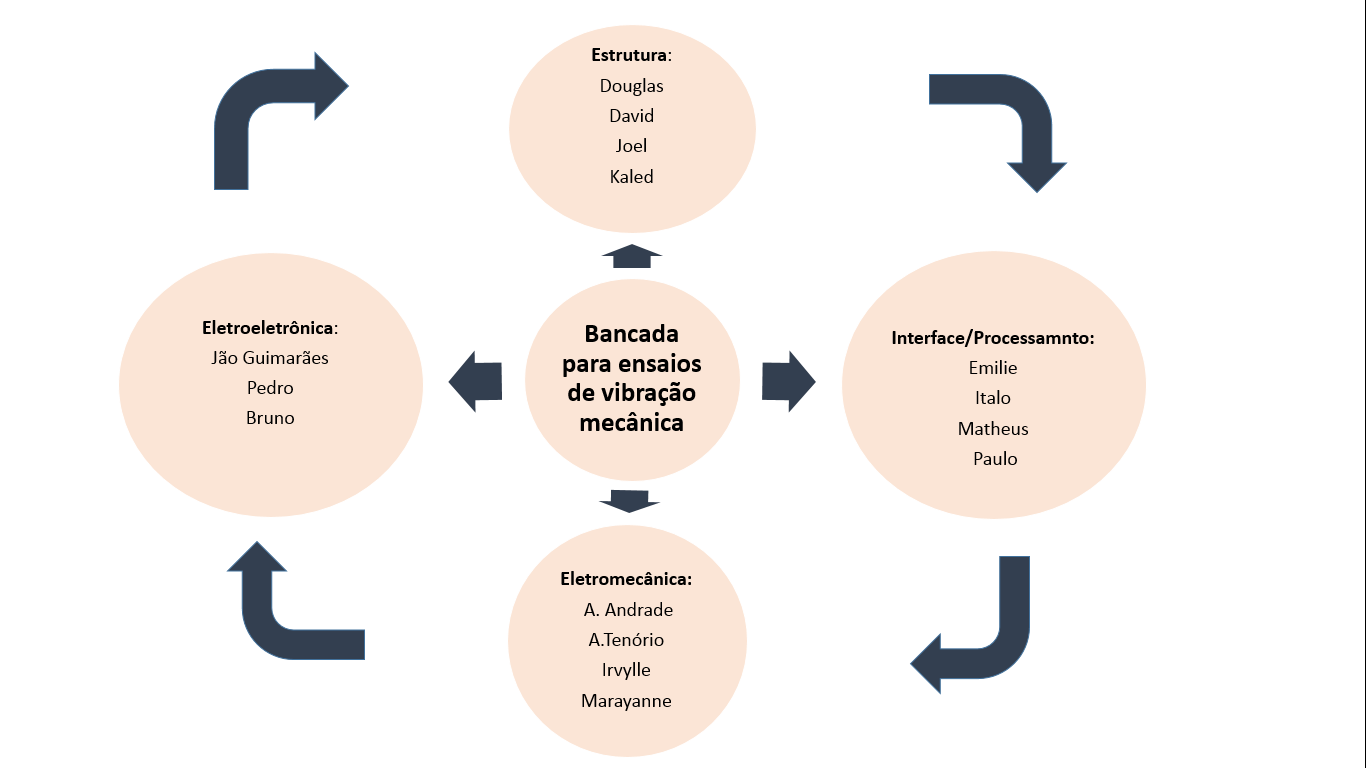
\includegraphics[keepaspectratio=true,scale=0.5]{figuras/organograma.png}
\caption{Organograma da equipe}
\label{organograma}
\end{figure} 

%%%%% CODIGO PRA FIGURA
% \begin{figure}[!ht]
% \centering
% \includegraphics[scale=0.6]{figuras/Organograma.png}
% \caption{Organograma do projeto}
% \label{Organograma}
% \end{figure}
%%%%%%%%%%%%%%%%%%%%%%%%%%%%%%%%%%%%%%%%%%%%%%%%%%%%%

\section*{Avaliação de resultados do projeto}
 Os sistemas de avaliação dos resultados do projeto são feitos a partir de reuniões ocorridas duas vezes na semana (quarta-feira e sexta-feira), nas quais são demonstradas e discutidas as evoluções até então, como também são definidos os próximos passos a serem dados, com base nas determinações já realizadas e nas orientações do que necessita ser feito.

\section*{Frequência da avaliação dos resultados do time}
Os resultados serão apresentados em reuniões com o time e posteriormente com toda a equipe durante as reuniões semanais. Os resultados também são divulgados nas plataformas de comunicação objetivando o esclarecimento de todos da equipe. 


%%%%%%%%%%%%%%%%%%%%%%% FIM PLANO DE GERENCIAMENTO DE RH

\chapter{Plano de Gerenciamento de Riscos}
  	\label{plano_de_riscos}
% 	\input{anexos/Plano_de_Gerenciamento_de_riscos}

%%%%%%%%%%%%%%%%%%%%%%% PLANO DE GERENCIAMENTO DE RISCOS

\begin{center}
 {\large Plano de gerenciamento de riscos}\\[0.2cm]
 {Bancada para Ensaios de Vibração Mecânica}\\
 \end{center}
 
 \section*{Histórico de Alterações}
\begin{table}[h]
\centering
\begin{tabular}{|c|c|p{6cm}|p{5cm}|}

Data & Versão & Descrição & Responsável\\
\hline                               
01/09/2016 & 1.0 & Criação do Plano de Gerenciamento de Riscos & Ítalo Paiva.
\\
\hline
\end{tabular}
\end{table}

\section*{Objetivo}
O objetivo desse plano é estabelecer um processo de gerenciamento de riscos do projeto e comunicar os riscos do projeto identificados.

\section*{Descrição dos processos de gerenciamento de riscos}

O Gerenciamento de Riscos possui processos definidos de seu planejamento, identificação, análise, planejamento de respostas e controle de riscos de um projeto \cite{pmbok}.
Para o plano de gerenciamento de riscos do projeto, os processos adotados serão os seguintes:

\begin{itemize}
  \item \textbf{Identificar os riscos} - processos de identificação de riscos que podem afetar o desenvolvimento do projeto.
  \item \textbf{Realizar a análise qualitativa dos riscos} - processo de priorização dos riscos identificados para avaliação de sua probabilidade de ocorrência e análise de seu impacto.
  \item \textbf{Planejar as respostas aos riscos} - processo que determina respostas às ocorrências de riscos para diminuir seu impacto e para reduzir ameaças às fases de desenvolvimento do projeto.
  \item \textbf{Controlar os riscos} - processo que acompanha e monitora os riscos identificados, identifica novos riscos e avalia a eficácia do processo de gerenciamento de riscos em todas as fases de desenvolvimento do projeto.
\end{itemize}

\section*{EAR – Estrutura Analítica de Riscos para identificação dos riscos}
	
  O Project Management Institute (PMI), criador do PMBoK, elaborou uma Estrutura Analítica de Riscos genérica para identificação dos riscos de um projeto a partir de categorias e subcategorias.
  \begin{figure}[h]
    \begin{center}
    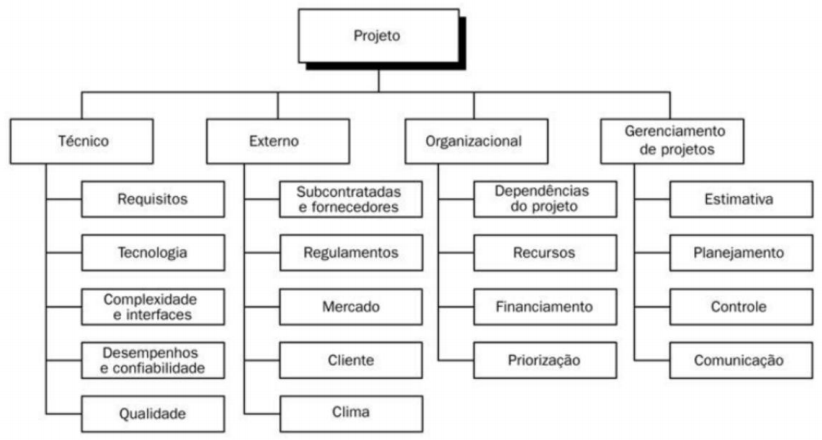
\includegraphics[scale=0.65]{figuras/ear_padrao.png}
    \label{ear_padrao}
    \end{center}
    \caption{Classificação dos riscos na EAR segundo o PMI}
  \end{figure}

As categorias e subcategorias foram analisadas em relação ao projeto e o resultado dessa análise está ilustrado nas Figuras \ref{riscos_tecnicos}, \ref{riscos_externos} e \ref{riscos_gerenciamento}.

  \begin{figure}[h]
    \begin{center}
    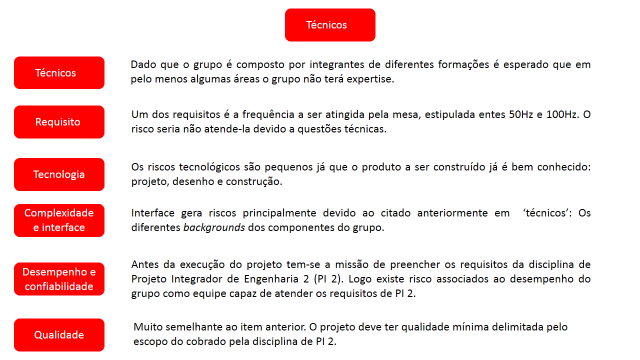
\includegraphics[scale=0.65]{figuras/riscos_tecnicos.png}
    \end{center}
    \label{riscos_tecnicos}
    \caption{Análise em relação aos riscos técnicos}
  \end{figure}
  
  \begin{figure}[h]
    \begin{center}
    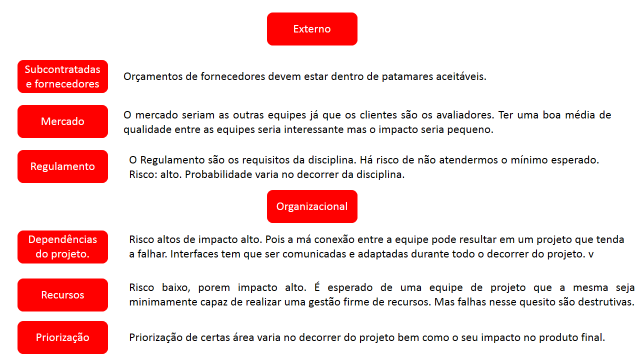
\includegraphics[scale=0.65]{figuras/riscos_externos_organizacional.png}
    \end{center}
    \label{riscos_externos}
    \caption{Análise em relação aos riscos externos e organizacionais}
  \end{figure}
  
  \begin{figure}[ht]
    \begin{center}
    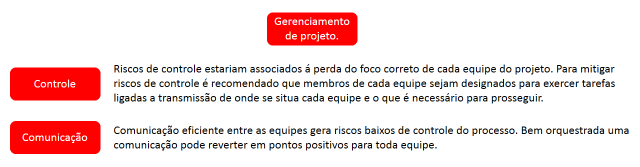
\includegraphics[scale=0.65]{figuras/riscos_gerenciamento.png}
    \end{center}
    \label{riscos_gerenciamento}
    \caption{Análise em relação aos riscos de gerenciamento}
  \end{figure}

\vfill
\pagebreak

\section*{Qualificação dos riscos}
Os riscos identificados serão qualificados na sua probabilidade de ocorrência e impacto nos resultados, conforme as Tabelas \ref{probabilidade_riscos} e \ref{impacto_riscos} ilustram.

\begin{table}[h]
\centering
\caption{Probabilidade dos riscos}
\label{probabilidade_riscos}
\begin{tabular}{|l|l|}
\hline
\multicolumn{1}{|c|}{\textbf{Nível}} & \multicolumn{1}{c|}{\textbf{Descrição}} \\ \hline
Baixo                                & Muito improvável (0\% - 30\%)       \\ \hline
Médio                                & Pouco provável (31\% - 60\%)            \\ \hline
Alto                                 & Provável (61\% - 90\%)                  \\ \hline
\end{tabular}
\end{table}


\begin{table}[h]
\centering
\caption{Impacto dos riscos}
\label{impacto_riscos}
\begin{tabular}{|l|l|}
\hline
\multicolumn{1}{|c|}{\textbf{Nível}} & \multicolumn{1}{c|}{\textbf{Descrição}} \\ \hline
Baixo & Tem pouco prejuízo ao desenvolvimento do projeto \\ \hline
Médio & Prejudica o desenvolvimento do projeto, mas de rápida resiliência \\ \hline
Alto & Tem muito prejuízo ao desenvolvimento do projeto \\ \hline
\end{tabular}
\end{table}

\subsection*{Prioridade dos riscos}

A prioridade dos riscos é dada pelo produto cartesiano da probabilidade e do impacto, conforme a Tabela \ref{prioridade_riscos}.

\begin{table}[h]
\centering
\caption{Classificação da Prioridade}
\label{prioridade_riscos}
\begin{tabular}{|
>{\columncolor[HTML]{9B9B9B}}c |
>{\columncolor[HTML]{34FF34}}c |c|
>{\columncolor[HTML]{FE0000}}c |}
\hline
\textbf{Provável} & \cellcolor[HTML]{FCFF2F}\textbf{Risco médio} & \cellcolor[HTML]{FE0000}\textbf{Risco alto} & \textbf{Risco extremo} \\ \hline
\textbf{Pouco provável} & \textbf{Risco baixo} & \cellcolor[HTML]{FCFF2F}\textbf{Risco médio} & \textbf{Risco alto} \\ \hline
\textbf{Muito improvável} & \textbf{Risco insignificante} & \cellcolor[HTML]{34FF34}\textbf{Risco baixo} & \cellcolor[HTML]{FCFF2F}\textbf{Risco médio} \\ \hline
\cellcolor[HTML]{656565}\textbf{Probabilidade/Impacto} & \cellcolor[HTML]{9B9B9B}\textbf{Baixo} & \cellcolor[HTML]{9B9B9B}\textbf{Médio} & \cellcolor[HTML]{9B9B9B}\textbf{Alto} \\ \hline
\end{tabular}
\end{table}

\subsection*{Riscos Identificados}

Os riscos identificados para o projeto estão listados na Tabela \ref{riscos_projeto}.

\begin{table}[h]
\centering
\caption{Riscos Identificados para o Projeto}
\label{riscos_projeto}
\begin{tabular}{|l|l|l|c|}
\hline
\multicolumn{1}{|c|}{\textbf{Risco}} & \multicolumn{1}{c|}{\textbf{Probabilidade}} & \multicolumn{1}{c|}{\textbf{Impacto}} & \textbf{Prioridade} \\ \hline
Algum membro abandonar a equipe & Baixa & Alto & \cellcolor[HTML]{FCFF2F}\textbf{Média} \\ \hline
Não houver financiamento suficiente. & Média & Alto & \cellcolor[HTML]{FE0000}\textbf{Alta} \\ \hline
\begin{tabular}[c]{@{}l@{}}Não conseguir os materiais\\  necessários para o produto por\\  tempo e localização.\end{tabular} & Baixa & Alto & \cellcolor[HTML]{FCFF2F}\textbf{Média} \\ \hline
Houver atrasos entre as equipes. & Média & Alto & \cellcolor[HTML]{FE0000}\textbf{Alta} \\ \hline
\begin{tabular}[c]{@{}l@{}}Os horários do galpão não serem\\  suficientes ou aptos.\end{tabular} & Alta & Médio & \cellcolor[HTML]{FE0000}\textbf{Alta} \\ \hline
\begin{tabular}[c]{@{}l@{}}Requisito entre as equipes serem\\ modificados no decorrer do processo.\end{tabular} & Média & Alto & \cellcolor[HTML]{FE0000}\textbf{Alta} \\ \hline
Greve & Baixa & Baixo & \cellcolor[HTML]{34FF34}\textbf{Baixa} \\ \hline
\end{tabular}
\end{table}

\subsection*{Ações de resposta aos riscos}

As ações definidas para reagir aos riscos identificados se encontram na Tabela \ref{acoes_riscos}.

\begin{table}[h]
\centering
\caption{Ações de contingência aos riscos}
\label{acoes_riscos}
\begin{tabular}{|c|c|}
\hline
\textbf{Risco} & \textbf{Ação de contingência} \\ \hline
Algum membro abandonar a equipe & \begin{tabular}[c]{@{}c@{}}Redistribuição de tarefas\\ 			e membros dentro da equipe\end{tabular} \\ \hline
Não houver financiamento suficiente & \begin{tabular}[c]{@{}c@{}}Modificação de parâmetros pontuais\\  com o objetivo de reduzir os custos\end{tabular} \\ \hline
\begin{tabular}[c]{@{}c@{}}Não conseguir os materiais\\  necessários para o produto por\\  tempo e localização\end{tabular} & \begin{tabular}[c]{@{}c@{}}Modificação de parâmetros pontuais com\\ o objetivo de adaptar o projeto a essa\\ 			situação, caso não encontre novos fornecedores\end{tabular} \\ \hline
Houver atrasos entre as equipes & \begin{tabular}[c]{@{}c@{}}Inicialmente,  comunicação\\ 			perante a equipe e busca de soluções internamente\\ 			\\ 			Em ultima instância,\\ 			comunicação aos professores da disciplina\end{tabular} \\ \hline
\begin{tabular}[c]{@{}c@{}}Os horários do galpão não serem\\  suficientes ou aptos\end{tabular} & \begin{tabular}[c]{@{}c@{}}Atividade será reposicionada para outro\\  local, na medida do possível\\  (local a definir com a equipe)\end{tabular} \\ \hline
\begin{tabular}[c]{@{}c@{}}Requisito entre as equipes serem\\ modificados no decorrer do processo\end{tabular} & \begin{tabular}[c]{@{}c@{}}Modificação de parâmetros pontuais\\ com o objetivo de adequar requisitos\end{tabular} \\ \hline
Greve & \begin{tabular}[c]{@{}c@{}}Os trabalhos continuarão e serão  readaptados\\  para os novos horários\end{tabular} \\ \hline
\end{tabular}
\end{table}

\section*{Sistema de Controle de mudanças de riscos}

Para controlar riscos e tentar de alguma forma amenizar percalços que possam atingir o projeto futuramente, o controle de riscos assume os problemas que possam surgir no decorrer do trabalho, de maneira que, caso aconteça algum risco não planejado, a resposta lógica da equipe será retornar ao documento de Gerenciamento de Risco, mensurar e analisar tal problema, assim como todos os outros, para que se possa tomar a medida mais adequada a situação.

\section*{Outros assuntos relacionados ao gerenciamento de riscos do projeto não previstos nesse plano}

Assuntos relacionados ao Gerenciamento de Riscos do Projeto que não foram previstos, caso aconteçam e mostrem relevância para o projeto, devem ser atualizados nesse documento, de maneira que este ande sempre alinhado com o projeto.

%%%%%%%%%%%%%%%%%%%%%%% FIM PLANO DE GERENCIAMENTO DE RISCOS

\chapter{Plano de Gerenciamento de Custos}
	\label{plano_de_custos}
% 	\input{anexos/Plano_de_Gerenciamento_de_Custos}
    
%%%%%%%%%%%%%%%%%%%%%%% PLANO DE GERENCIAMENTO DE CUSTOS

\begin{center}
 {\large Plano de Gerenciamento de Custos}\\[0.2cm]
 {Bancada para Ensaios de Vibração Mecânica}\\
 \end{center}
 
 \section*{Histórico de Alterações}
\begin{table}[h]
\centering
\begin{tabular}{|c|c|p{6cm}|p{5cm}|}

Data & Versão & Descrição & Responsável\\
\hline                               
01/09/2016 & 1.0 & Criação deste documento & Emilie Morais\\ \hline
\end{tabular}
\end{table}

\section*{Objetivo}
  O objetivo desse plano é definir como será realizado o gerenciamento de custos do projeto, bem como apresentar o custo total estimado.

  
\section*{Descrição dos processos de gerenciamento de custo}

Primeiramente, será realizada a estimativa do custo de aquisições do projeto, pois dado o contexto do projeto não será calculado o custo de mão-de-obra. A partir do custo estimado será definido o orçamento do projeto, considerando cada integrante.

Durante a execução do projeto os custos serão monitorados a fim de visualizar o custo planejado e o custo real.

% Considerando a solução proposta no projeto foram estabelecidos os materiais que serão utilizados para a construção da bancada, considerando também os componentes eletrônicos e serviço de hospedagem. 
% Para cada material foi pesquisado um valor e dessa forma o custo total do projeto foi estimado. 

% para ter base da viabilidade do projeto e que seu custo não ultrapasse o estabelecido no orçamento do projeto.

\section*{Alocação financeira das mudanças no orçamento}

As mudanças serão comunicadas ao grupo que decidirá sobre o orçamento disponível.

%%%%%%%%%%%%%%%%%%%%%%% FIM PLANO DE GERENCIAMENTO DE CUSTOS
    
\chapter{Plano de Gerenciamento de Aquisições}
	\label{plano_de_aquisicoes}    						
% 	\input{anexos/Plano_de_Gerenciamento_de_aquisicoes}

%%%%%%%%%%%%%%%%%%%%%%% PLANO DE GERENCIAMENTO DE AQUISIÇÕES

\begin{center}
 {\large Plano de gerenciamento de Aquisições}\\[0.2cm]
 {Bancada para Ensaios de Vibração Mecânica}\\
 \end{center}
 
 \section*{Histórico de Alterações}
\begin{table}[h]
\centering
\begin{tabular}{|c|c|p{6cm}|p{5cm}|}

Data & Versão & Descrição & Responsável\\
\hline                               
28/08/2016 & 1.0 & Criação do Plano de Gerenciamento de Aquisições & Emilie Morais\\
\hline
\end{tabular}
\end{table}

\section*{Objetivo}
  O objetivo desse plano é definir como será realizado o gerenciamento de aquisições do projeto.
  
\section*{Descrição do processo de gerenciamento das aquisições}
 A partir dos requisitos do projeto serão estabelecidos os itens necessários a serem adquiridos. Para cada produto será estipulada uma data na qual o produto deve estar disponível para o projeto. 
 
Considerando essa data, haverá a solicitação de aquisição pelo líder da área. Caso o item solicitado não tenha sido previsto no início do projeto a necessidade de aquisição será verificada. 

Após a aprovação da solicitação pelo grupo, o fornecedor será escolhido, o recurso financeiro será alocado e a aquisição será efetivada.

\section*{Gerenciamento e formas de aquisição}
As formas de aquisição dos produtos/serviços serão:
\begin{itemize}
	\item Compra imediata;
    \item Encomenda;
    \item Empréstimo;
    \item Contrato mensal;
\end{itemize}
Para os produtos de compra imediata e encomenda a compra será efetuada no valor total do produto e para o serviço de hospedagem do software será feito um plano gratuito de 3 meses para realização do projeto. Para uso do sistema após o término do projeto, a hospedagem passará a ter um valor fixo por mês.

\section*{Critérios de avaliação de cotações e propostas}
\label{criterios}
A escolha dos fornecedores será realizada considerando custo-benefício do produto ou serviço e a viabilidade de entrega no prazo necessário para o projeto.   

\section*{Alocação financeira para as aquisições}
Considerando o custo total estimado do projeto de R\$ 3.253,87, este será dividido igualitariamente entre os membros da equipe do projeto. Para cada produto que for necessário adquirir será estipulada uma data para compra e o valor será requisitado aos membros da equipe.

\section*{Responsáveis pelas Aquisições}
A responsabilidade pela aquisição será dividida por área, sendo:

\begin{itemize}
	\item Frente de Estrutura - João Kaled\\
	\item Frente Eletroeletrônica - Pedro Henrique Gonçalves Inazawa\\
	\item Frente Eletromecânica - Anderson Andrade Barbosa\\
	\item Frente Interface/Processamento - Matheus Herlan dos Santos Ferraz\\
\end{itemize}

%%%%%%%%%%%%%%%%%%%%%%% FIM PLANO DE GERENCIAMENTO DE AQUISIÇÕES

\chapter{Cronograma Detalhado}
	\label{cronograma_detalhado}
%     

\chapter{Cronograma Detalhado}
	\label{cronograma_detalhado}
%     

\chapter{Cronograma Detalhado}
	\label{cronograma_detalhado}
%     

\chapter{Cronograma Detalhado}
	\label{cronograma_detalhado}
%     \input{anexos/cronograma_detalhado}

%%%%%%%%%%%%%%%%%%%%%%% CRONOGRAMA DETALHADO

\begin{figure}[!ht]
\centering
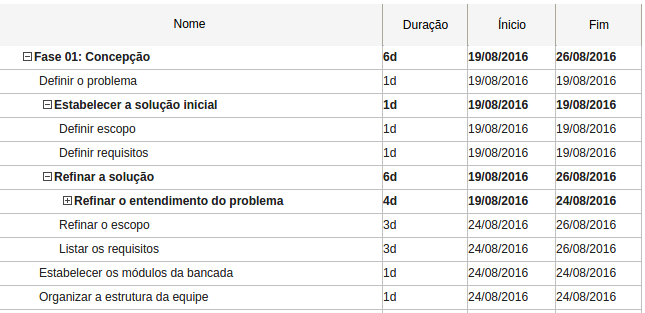
\includegraphics[scale=1]{figuras/cronograma_fase01.png}
\caption{Cronograma da Fase 01 - Concepção}
\end{figure}

\begin{figure}[!ht]
\centering
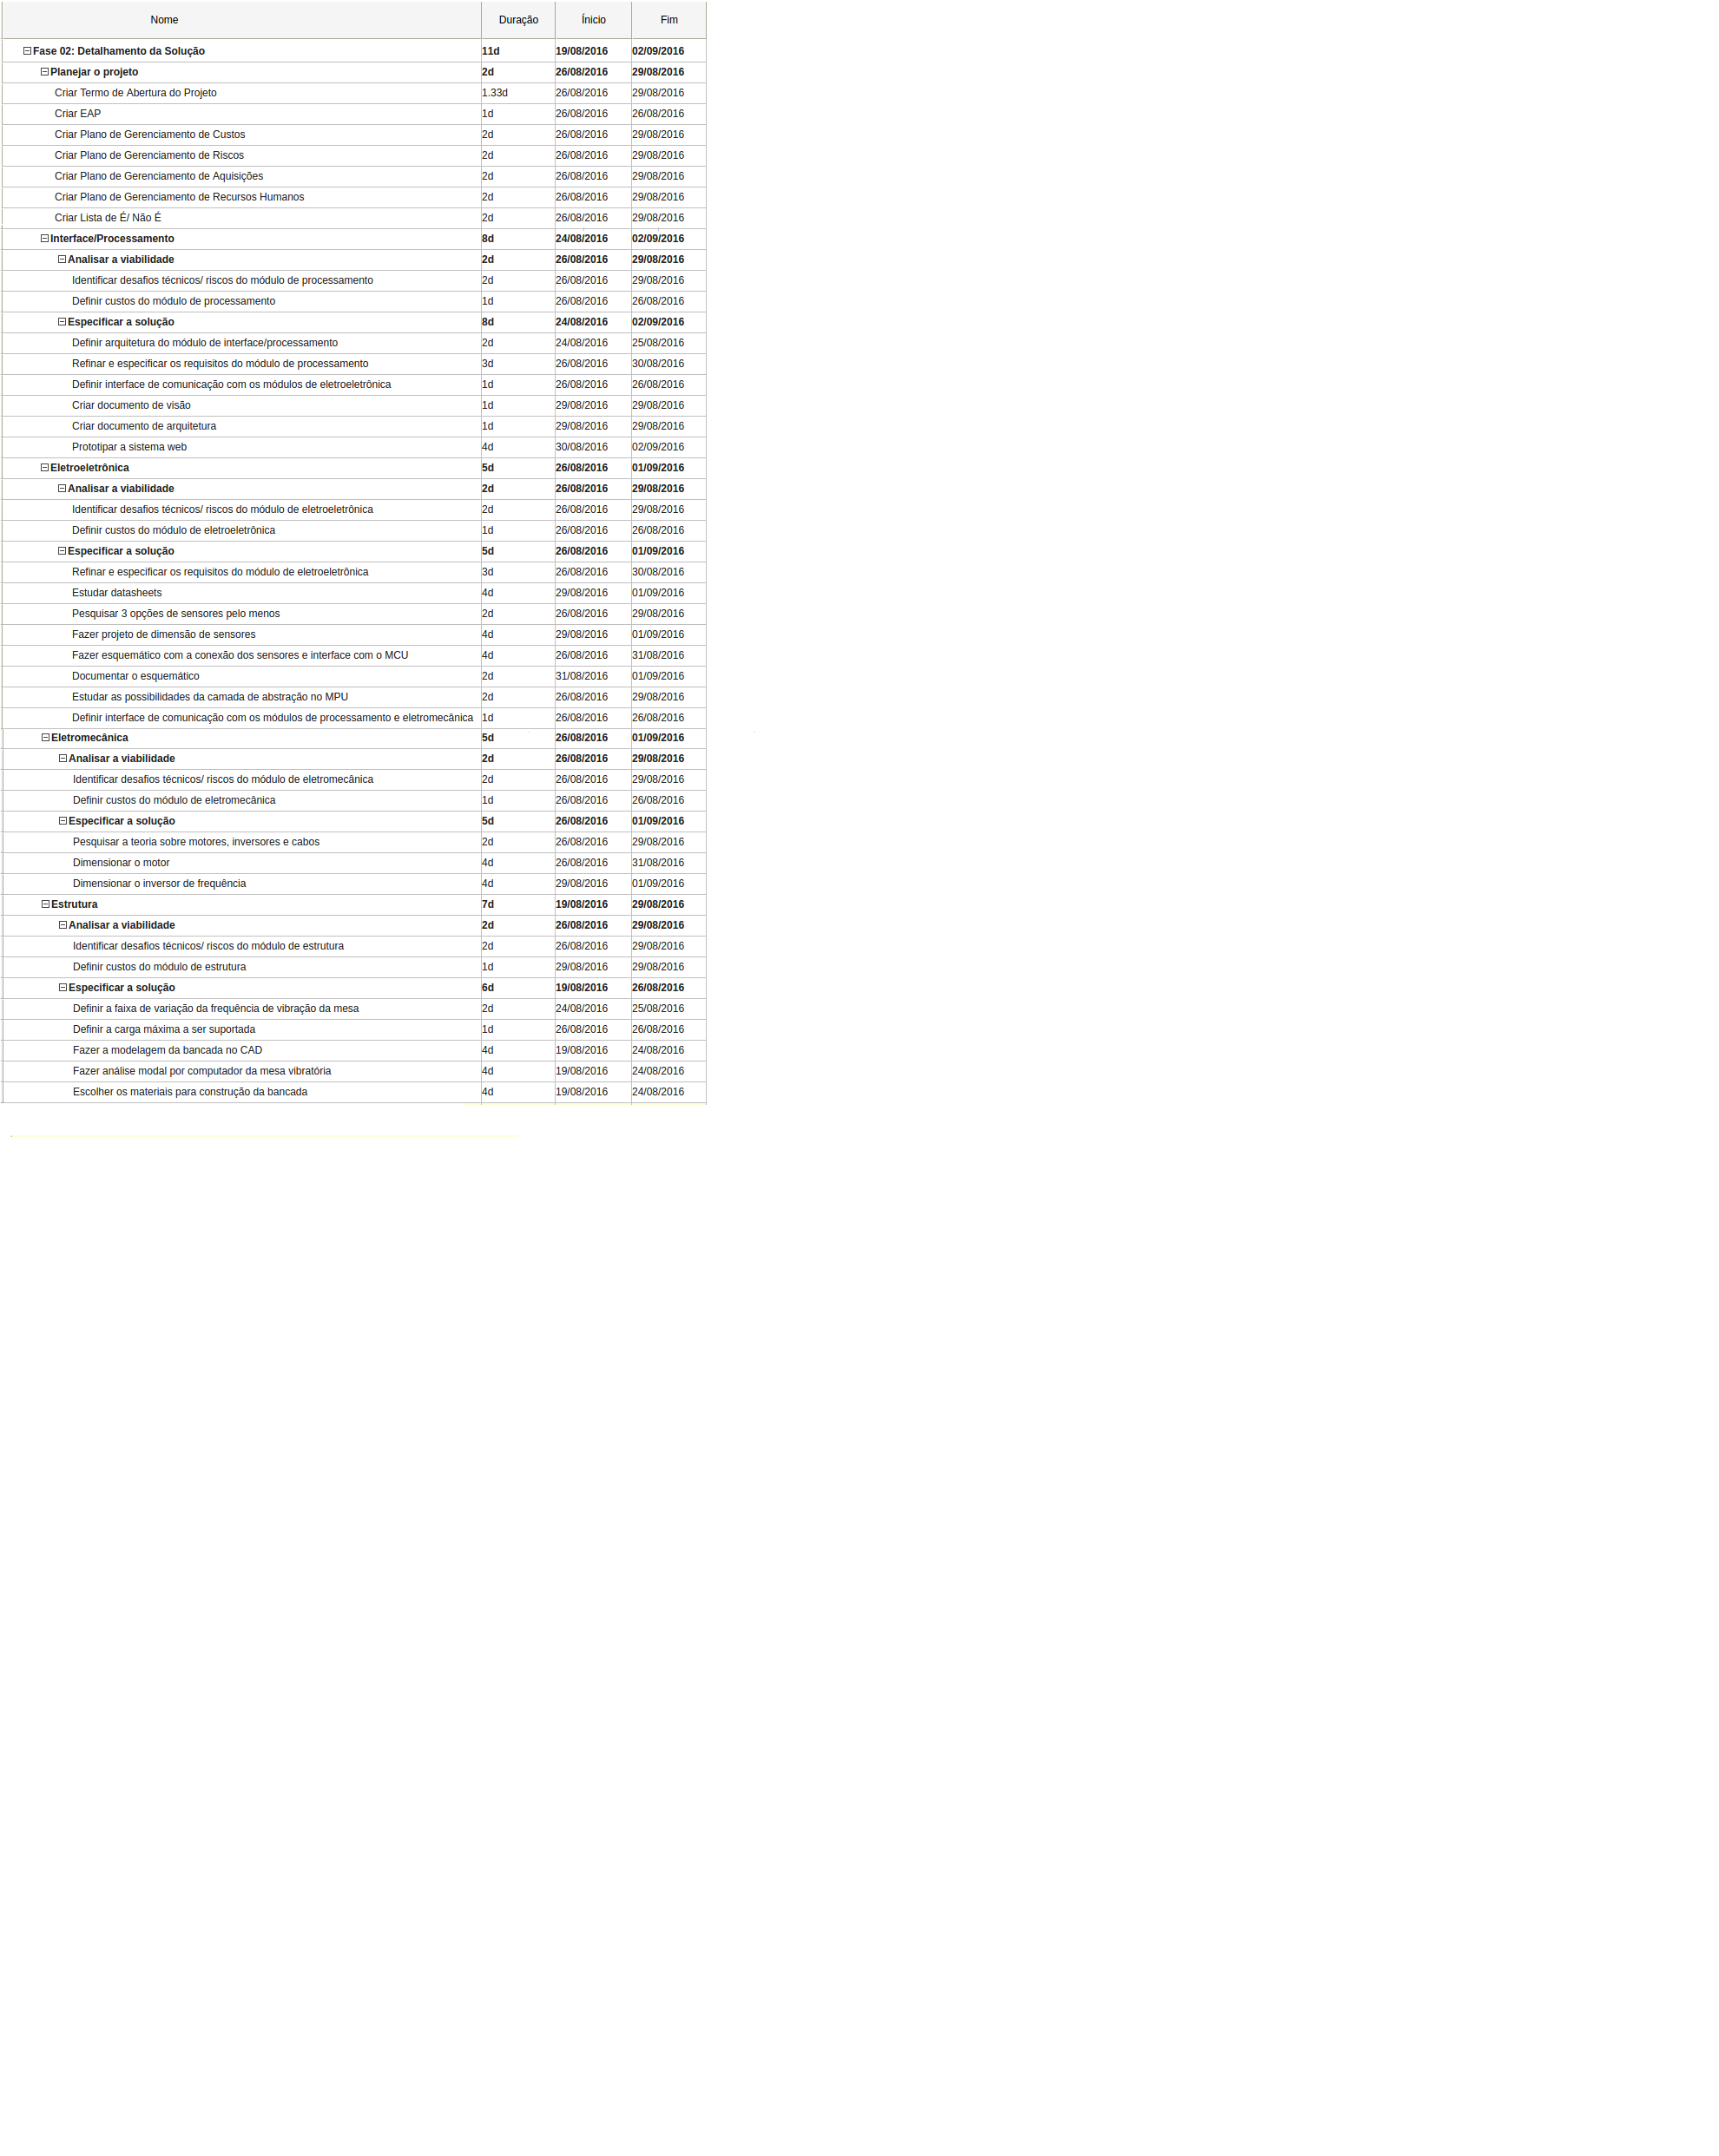
\includegraphics[scale=0.6]{figuras/cronograma_fase02.png}
\caption{Cronograma da Fase 02 - Detalhamento da Solução}
\end{figure}

\begin{figure}[!ht]
\centering
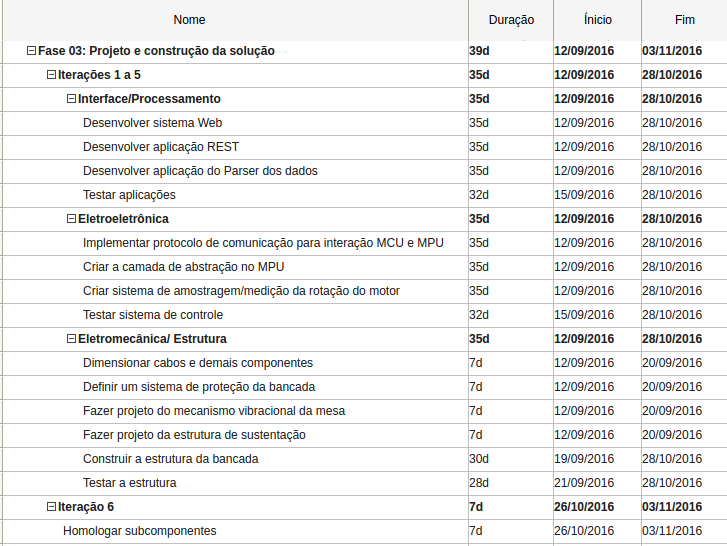
\includegraphics[scale=0.9]{figuras/cronograma_fase03.png}
\caption{Cronograma da Fase 03 - Projeto e Construção}
\end{figure}

\begin{figure}[!ht]
\centering
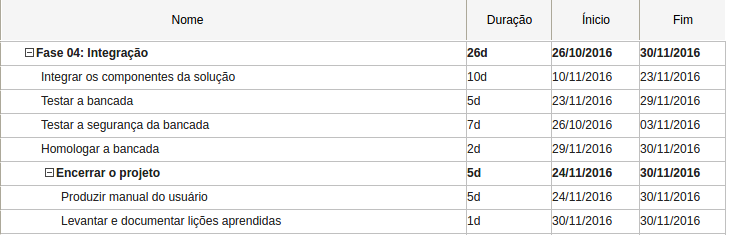
\includegraphics[scale=0.9]{figuras/cronograma_fase04.png}
\caption{Cronograma da Fase 04 - Integração}
\end{figure}
\vfill
\pagebreak

%%%%%%%%%%%%%%%%%%%%%%% FIM CRONOGRAMA DETALHADO

%%%%%%%%%%%%%%%%%%%%%%% CRONOGRAMA DETALHADO

\begin{figure}[!ht]
\centering
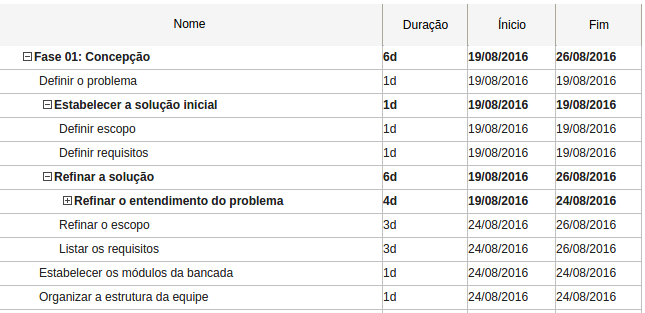
\includegraphics[scale=1]{figuras/cronograma_fase01.png}
\caption{Cronograma da Fase 01 - Concepção}
\end{figure}

\begin{figure}[!ht]
\centering
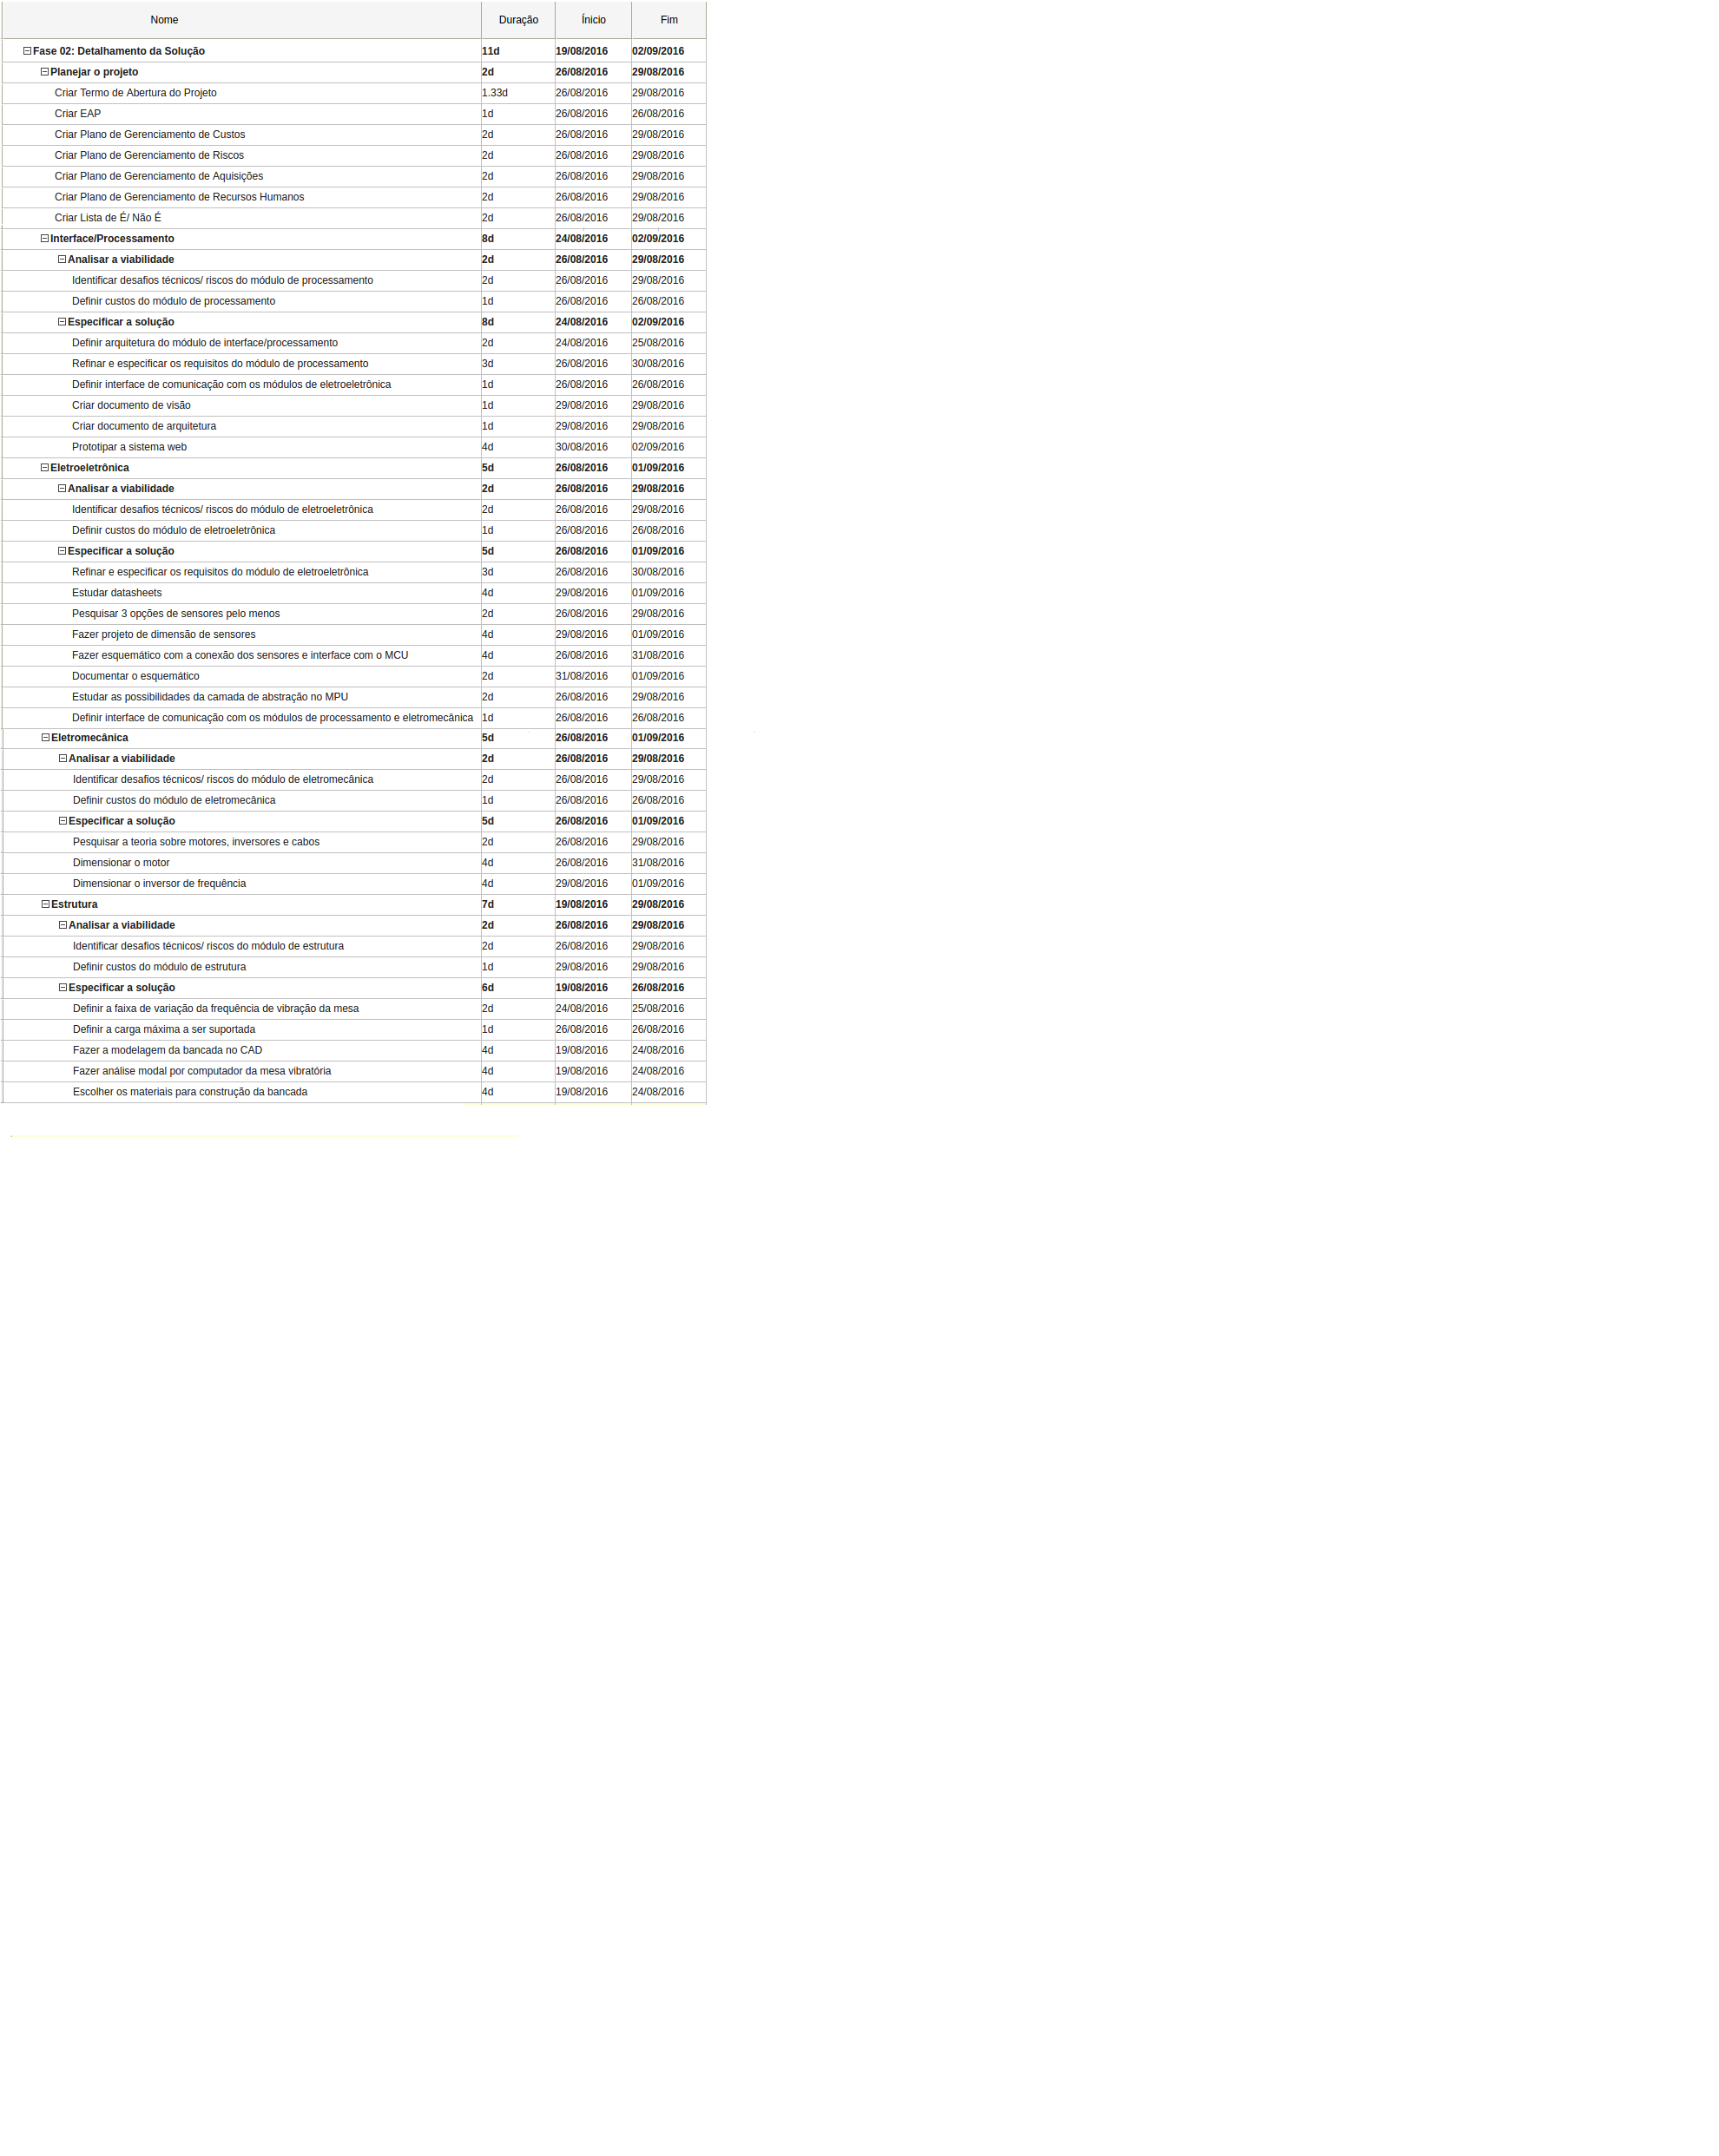
\includegraphics[scale=0.6]{figuras/cronograma_fase02.png}
\caption{Cronograma da Fase 02 - Detalhamento da Solução}
\end{figure}

\begin{figure}[!ht]
\centering
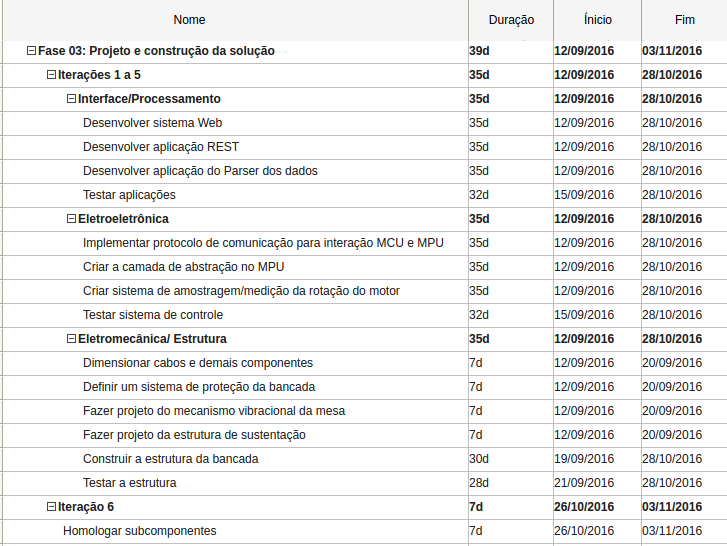
\includegraphics[scale=0.9]{figuras/cronograma_fase03.png}
\caption{Cronograma da Fase 03 - Projeto e Construção}
\end{figure}

\begin{figure}[!ht]
\centering
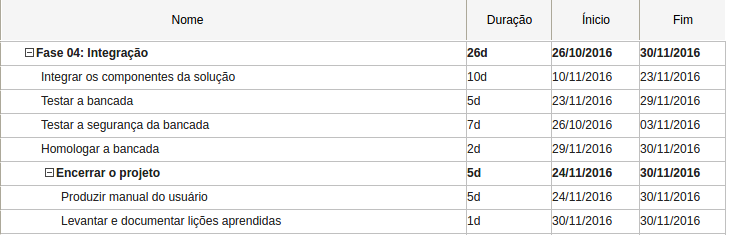
\includegraphics[scale=0.9]{figuras/cronograma_fase04.png}
\caption{Cronograma da Fase 04 - Integração}
\end{figure}
\vfill
\pagebreak

%%%%%%%%%%%%%%%%%%%%%%% FIM CRONOGRAMA DETALHADO

%%%%%%%%%%%%%%%%%%%%%%% CRONOGRAMA DETALHADO

\begin{figure}[!ht]
\centering
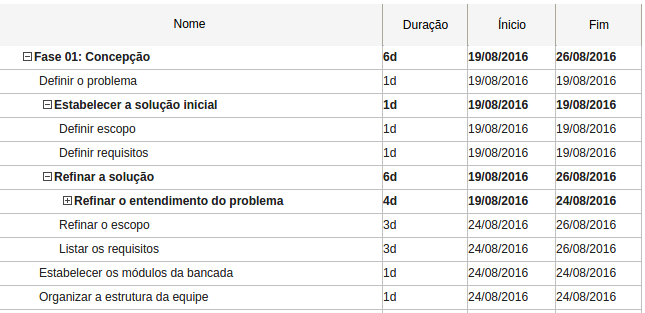
\includegraphics[scale=1]{figuras/cronograma_fase01.png}
\caption{Cronograma da Fase 01 - Concepção}
\end{figure}

\begin{figure}[!ht]
\centering
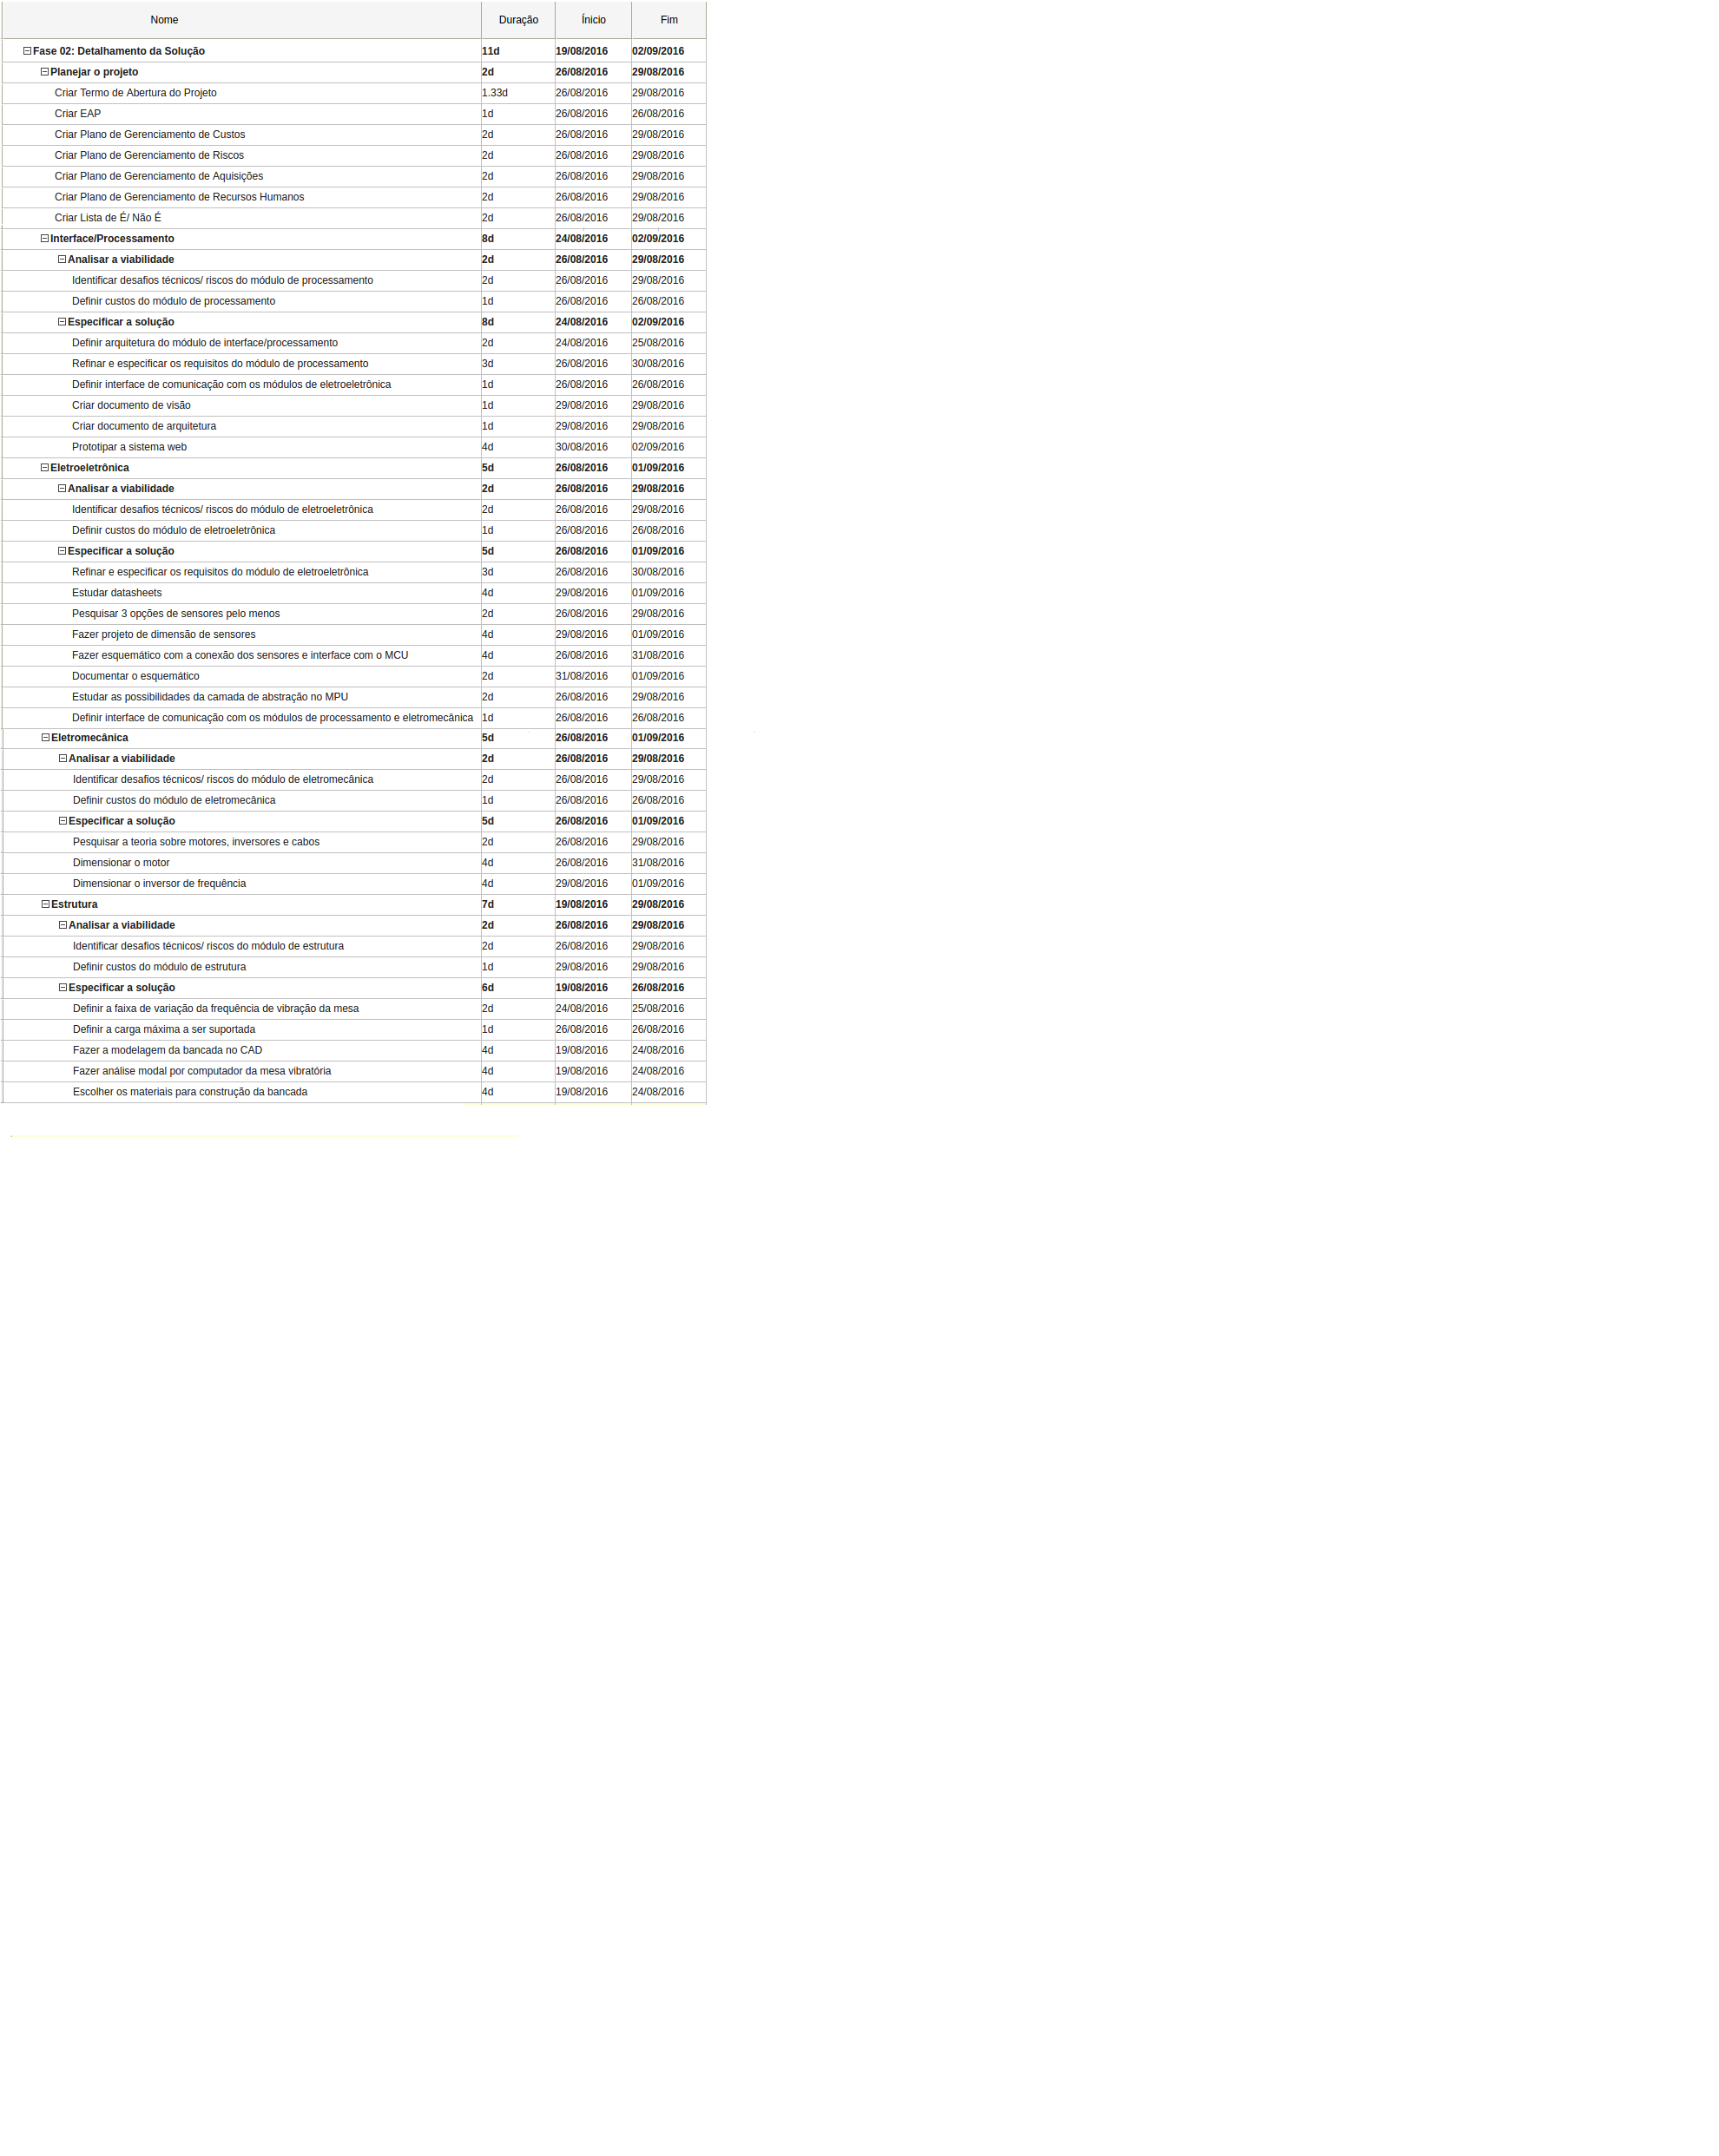
\includegraphics[scale=0.6]{figuras/cronograma_fase02.png}
\caption{Cronograma da Fase 02 - Detalhamento da Solução}
\end{figure}

\begin{figure}[!ht]
\centering
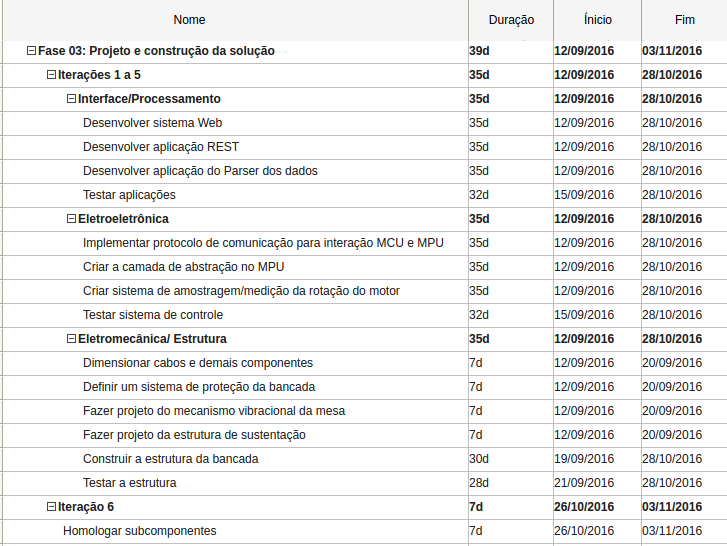
\includegraphics[scale=0.9]{figuras/cronograma_fase03.png}
\caption{Cronograma da Fase 03 - Projeto e Construção}
\end{figure}

\begin{figure}[!ht]
\centering
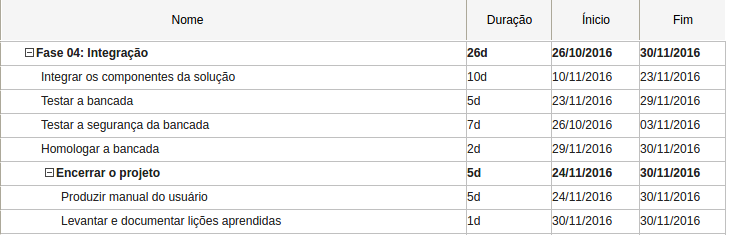
\includegraphics[scale=0.9]{figuras/cronograma_fase04.png}
\caption{Cronograma da Fase 04 - Integração}
\end{figure}
\vfill
\pagebreak

%%%%%%%%%%%%%%%%%%%%%%% FIM CRONOGRAMA DETALHADO

%%%%%%%%%%%%%%%%%%%%%%% CRONOGRAMA DETALHADO

\begin{figure}[!ht]
\centering
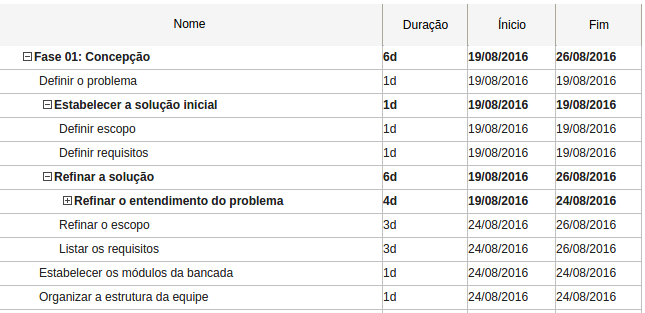
\includegraphics[scale=1]{figuras/cronograma_fase01.png}
\caption{Cronograma da Fase 01 - Concepção}
\end{figure}

\begin{figure}[!ht]
\centering
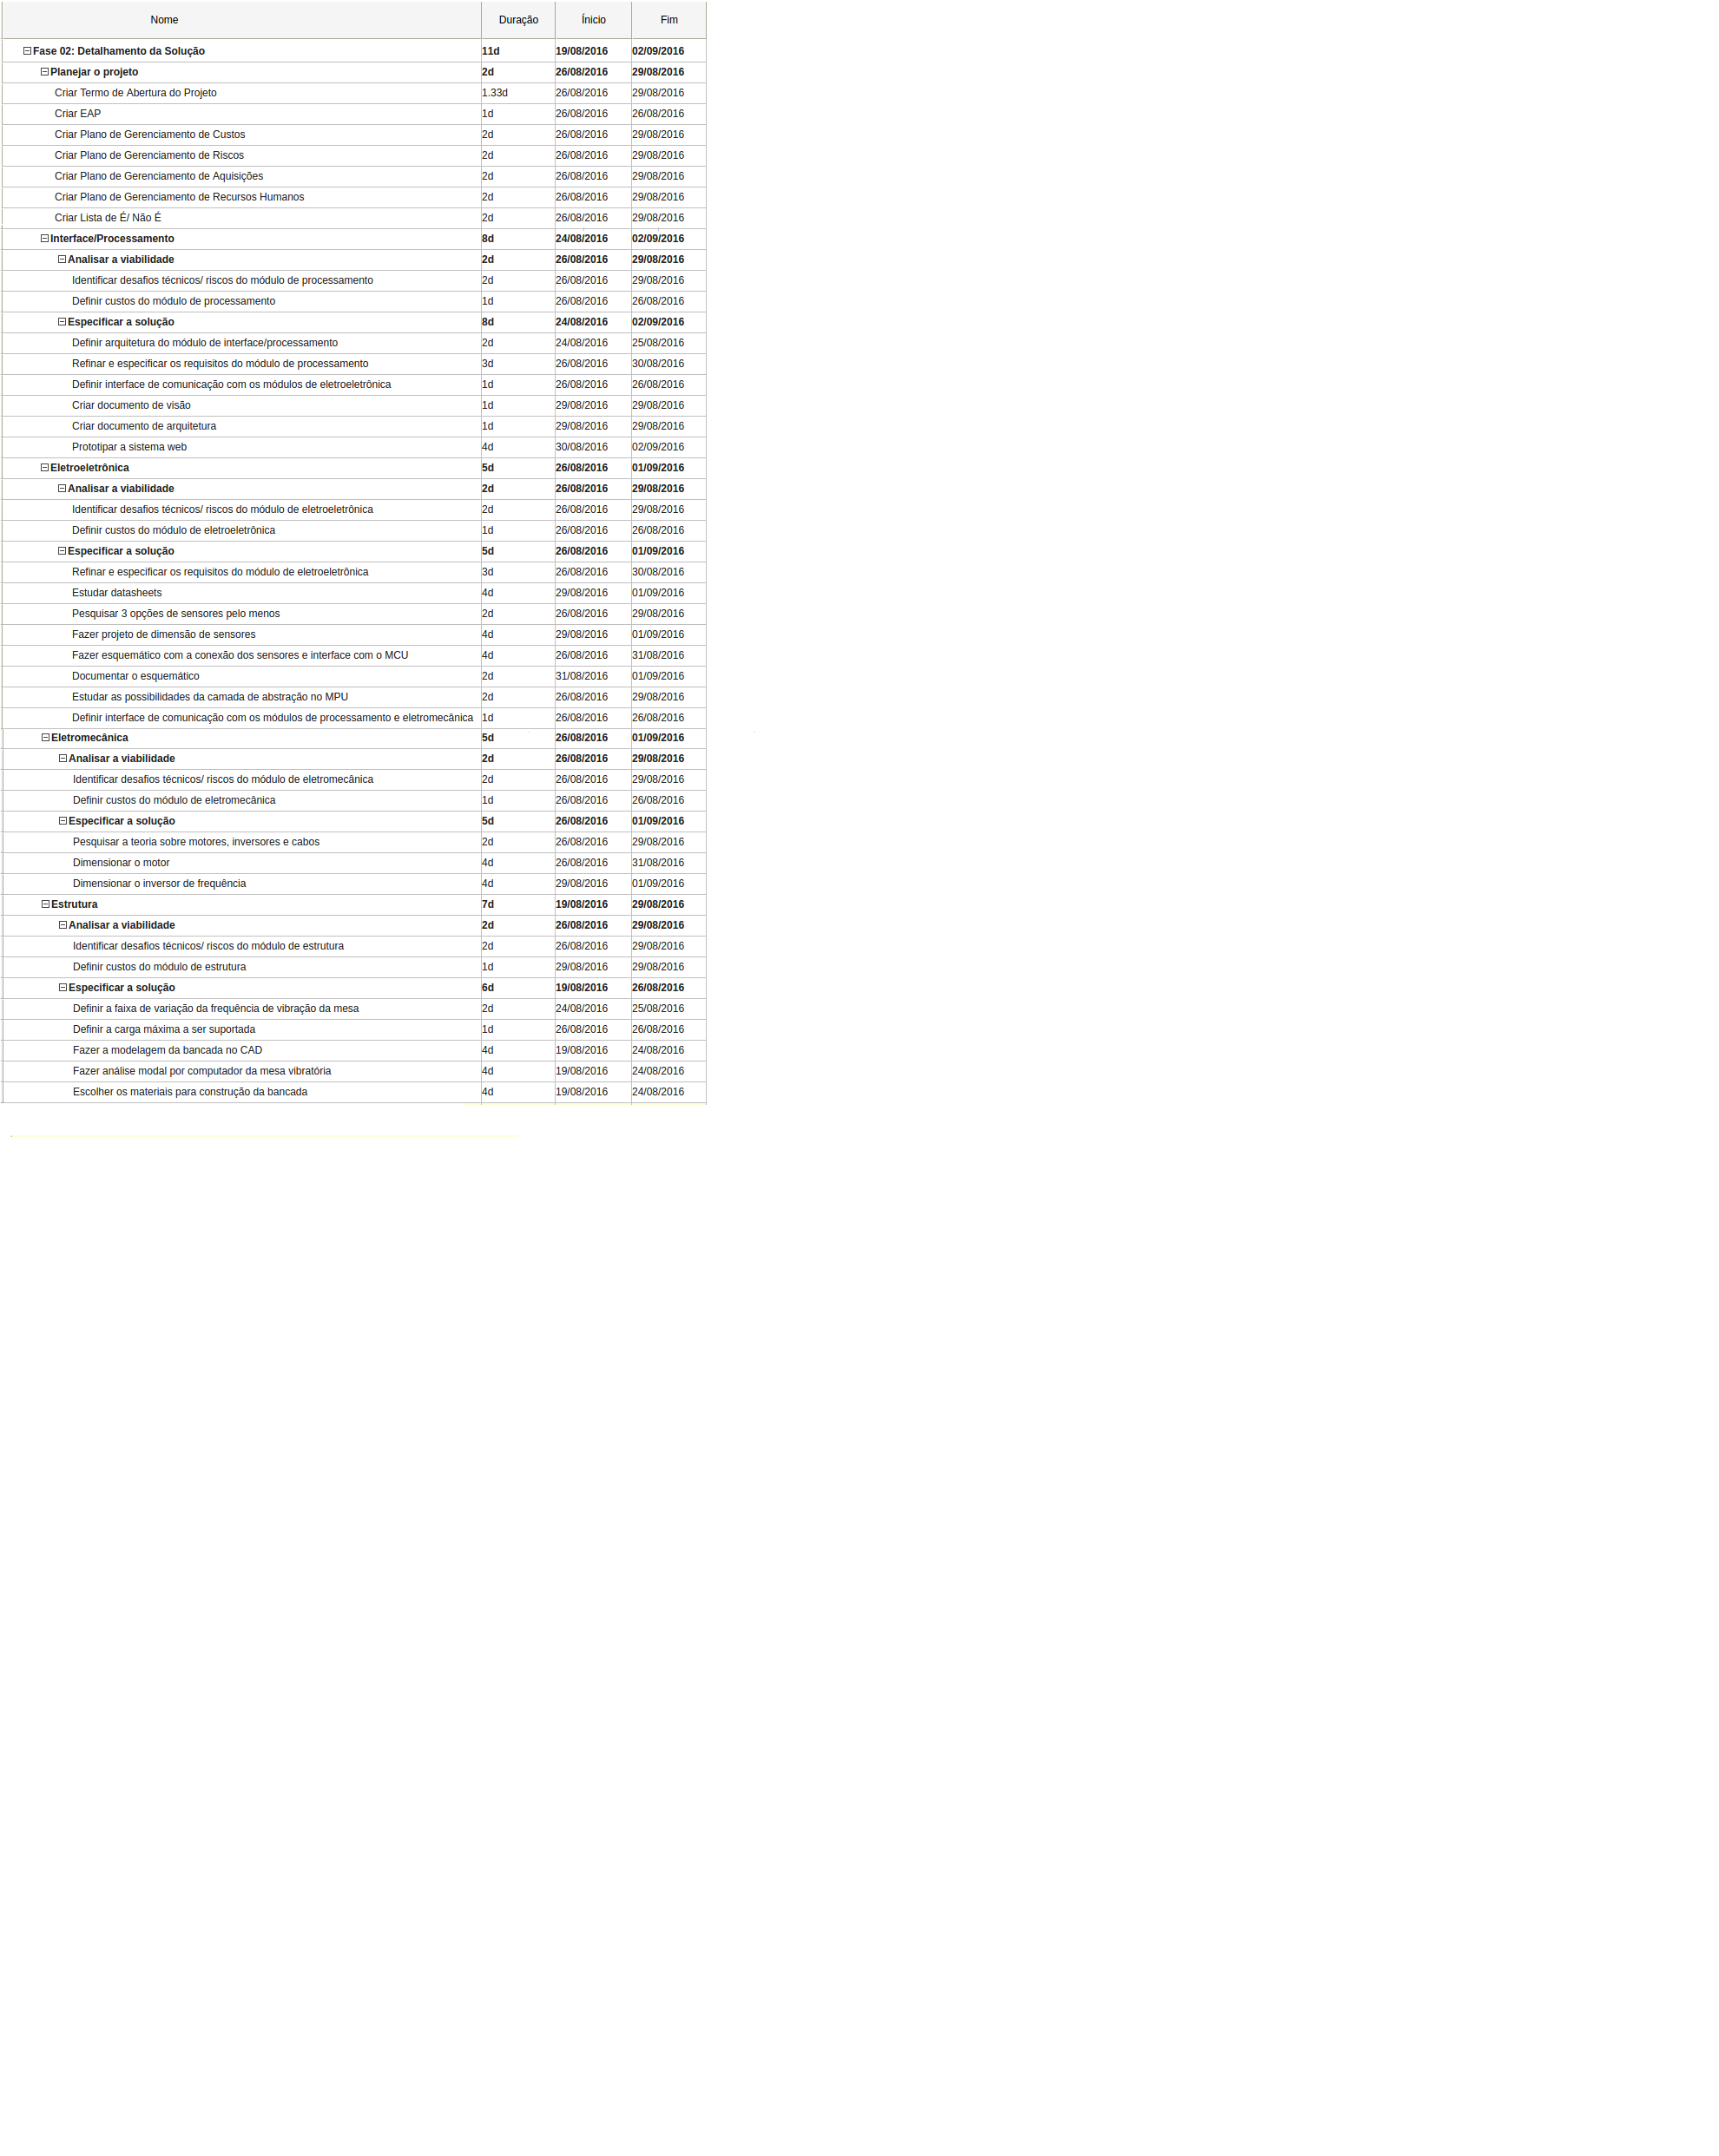
\includegraphics[scale=0.75]{figuras/cronograma_fase02.png}
\caption{Cronograma da Fase 02 - Detalhamento da Solução}
\end{figure}

\begin{figure}[!ht]
\centering
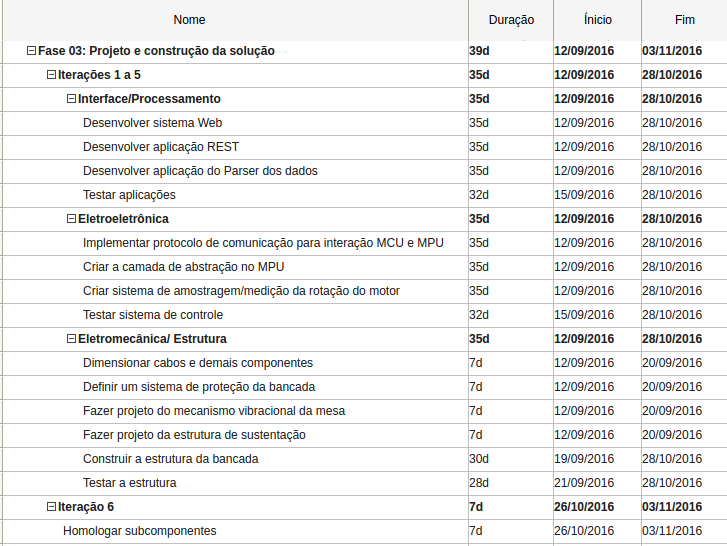
\includegraphics[scale=0.9]{figuras/cronograma_fase03.png}
\caption{Cronograma da Fase 03 - Projeto e Construção}
\end{figure}

\begin{figure}[!ht]
\centering
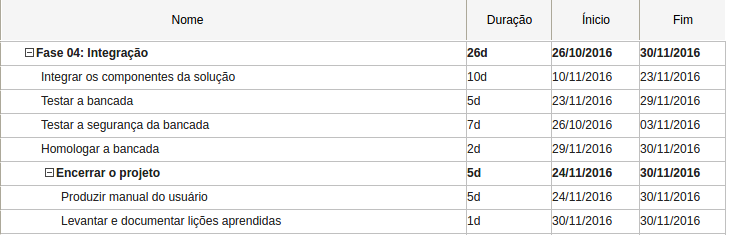
\includegraphics[scale=0.9]{figuras/cronograma_fase04.png}
\caption{Cronograma da Fase 04 - Integração}
\end{figure}

%%%%%%%%%%%%%%%%%%%%%%% FIM CRONOGRAMA DETALHADO

\chapter{Documento de Visão do Sistema Web}
% 	\input{anexos/Documento_de_visao}

%%%%%%%%%%%%%%%%%%%%%%% DOC DE VISÃO

\begin{center}
 {\large Documento de Visão}\\[0.2cm]
 {BEViM}\\
 \end{center}
 
 \section*{Histórico de Alterações}
\begin{table}[h]
\centering
\begin{tabular}{|c|c|p{6cm}|p{5cm}|}
\hline
Data & Versão & Descrição & Responsável\\
\hline                               
27/08/2016 & 1.0 & Criação do documento. & Ítalo Paiva e Emilie Morais.\\
\hline
\end{tabular}
\end{table}

\section*{Introdução}
	
    O objetivo deste documento é estabelecer uma visão geral do BEViM, que é o sistema que será utilizado para controle e visualização dos resultados da bancada para ensaios de vibração mecânica. Dessa forma, este documento apresenta as necessidades macro do usuário, características gerais do software e envolvidos.
    
   
\section*{Descrições dos Envolvidos e dos Usuários}
	
    Nesta seção do documento são apresentados os envolvidos, os usuários e suas principais necessidades e o ambiente de uso do sistema.
    \subsection*{Resumo dos envolvidos}
		
        Os envolvidos no projeto seja no desenvolvimento, na aquisição ou no uso da aplicação final são \textit{stakeholders}. Foram considerados envolvidos no projeto todos que tenham algum tipo de interesse e/ou participação, e a Tabela \ref{soft_stakeholders} lista os \textit{stakeholders} identificados.

\vfill
\pagebreak
        \begin{table}[h]
            \centering
            \caption{Envolvidos do projeto de Software}
            \label{soft_stakeholders}
            \begin{tabular}{|c|c|c|}
            \hline
            \textbf{Nome}      & \textbf{Descrição}                                                                            & \textbf{Responsabilidades}                                                                                                              \\ \hline
            Emilie Morais      & \begin{tabular}[c]{@{}c@{}}Membro do time\\  de desenvolvimento\end{tabular}                  & Desenvolver e manter o sistema                                                                                                          \\ \hline
            Ítalo Paiva        & \begin{tabular}[c]{@{}c@{}}Membro do time\\  de desenvolvimento\end{tabular}                  & Desenvolver e manter o sistema                                                                                                          \\ \hline
            Matheus Ferraz     & \begin{tabular}[c]{@{}c@{}}Membro do time\\  de desenvolvimento\end{tabular}                  & Desenvolver e manter o sistema                                                                                                          \\ \hline
            Paulo Borba        & \begin{tabular}[c]{@{}c@{}}Membro do time\\  de desenvolvimento\end{tabular}                  & Desenvolver e manter o sistema                                                                                                          \\ \hline
            Demais integrantes & \begin{tabular}[c]{@{}c@{}}Integrantes do grupo de\\  desenvolvimento da bancada\end{tabular} & \begin{tabular}[c]{@{}c@{}}Acompanhar o desenvolvimento \\ e validar a integração do software\\  com os demais subprodutos\end{tabular} \\ \hline
            Professores de PI2 & Professor da disciplina de PI2                                                                & \begin{tabular}[c]{@{}c@{}}Monitorar o andamento do projeto; \\ Avaliar o projeto e o produto.\end{tabular}                             \\ \hline
            \begin{tabular}[c]{@{}c@{}}Alunos \\ (Automotiva e/ou Aeroespacial)\end{tabular} & \begin{tabular}[c]{@{}c@{}}Usuário direto\\  do sistema\end{tabular} & \begin{tabular}[c]{@{}c@{}}Realizar testes no equipamento,\\  controlando a bancada.\end{tabular} \\ \hline
          Técnicos & \begin{tabular}[c]{@{}c@{}}Usuário direto \\ do sistema\end{tabular} & \begin{tabular}[c]{@{}c@{}}Gerenciar e acompanhar \\ o uso do equipamento.\end{tabular} \\ \hline
          \begin{tabular}[c]{@{}c@{}}Professores \\ (Automotiva e/ou Aeroespacial)\end{tabular} & \begin{tabular}[c]{@{}c@{}}Usuário direto\\ do sistema\end{tabular} & \begin{tabular}[c]{@{}c@{}}Realizar testes no equipamento,\\  controlando a bancada\end{tabular} \\ \hline
            \end{tabular}
        \end{table}
        
    \subsection*{Resumo dos usuários}\label{resumo_usuarios_secao}
    
    	Na tabela \ref{usuarios_resumo} estão listados os usuários do sistema.
    
    	\begin{table}[h]
          \centering
          \caption{Resumo dos usuários do sistema}
          \label{usuarios_resumo}
          \begin{tabular}{|c|c|c|}
          \hline
          \textbf{Nome} & \textbf{Descrição} & \textbf{Responsabilidades} \\ \hline
          \begin{tabular}[c]{@{}c@{}}Alunos \\ (Automotiva e/ou Aeroespacial)\end{tabular} & \begin{tabular}[c]{@{}c@{}}Usuário direto\\  do sistema\end{tabular} & \begin{tabular}[c]{@{}c@{}}Realizar testes no equipamento,\\  controlando a bancada.\end{tabular} \\ \hline
          Técnicos & \begin{tabular}[c]{@{}c@{}}Usuário direto \\ do sistema\end{tabular} & \begin{tabular}[c]{@{}c@{}}Gerenciar e acompanhar \\ o uso do equipamento.\end{tabular} \\ \hline
          \begin{tabular}[c]{@{}c@{}}Professores \\ (Automotiva e/ou Aeroespacial)\end{tabular} & \begin{tabular}[c]{@{}c@{}}Usuário direto\\ do sistema\end{tabular} & \begin{tabular}[c]{@{}c@{}}Realizar testes no equipamento,\\  controlando a bancada\end{tabular} \\ \hline
          \end{tabular}
    	\end{table}
    
     \subsection*{Principais necessidades do usuário}
     As necessidades, dos alunos e professores, a serem solucionadas pelo sistema são:
     \begin{itemize}
		\item Iniciar um ensaio na bancada controlando a frequência e o tempo de vibração;
        \item Visualizar os dados de amplitude, frequência, tempo na bancada e no objeto testado;
        \item Obter dados de testes já realizados;
%         \item Agendar horário de uso da bancada;	
    \end{itemize}
    
%     A necessidade, dos técnicos, a ser solucionada pelo sistema é:
%      \begin{itemize}
%         \item Controlar o uso da bancada;
%     \end{itemize}
     
	\subsection*{Ambiente do usuário}
    	
        Os usuários principais são os alunos de Engenharia Automotiva e Aeroespacial e os técnicos, que utilizarão o sistema nos laboratórios da FGA. Como o sistema é uma aplicação \textit{Web}, é possível acessá-lo de qualquer lugar com uma conexão com a Internet.
        
   
\section*{Visão geral do produto}

	\subsection*{Perspectiva e Intenção do produto}
    	Espera-se que o \textit{software} facilite o uso da bancada de ensaios, permitindo um controle mais fácil e uma visualização mais agradável e cômoda dos resultados dos testes, simplificando a vida dos alunos.
        
    \subsection*{Funcionalidades do produto}
    
    	As funcionalidades são um conjunto de características e comportamentos que o sistema deve conter para resolver o problema e as necessidades do cliente. O software BEViM conta com as seguintes funcionalidades:
        
        \begin{itemize}
          	\item \textbf{Controle da bancada} - Esta funcionalidade permite que o usuário controle a entrada de dados para realizar um ensaio de vibração na bancada.
            \item \textbf{Visualização dos resultados} - Esta funcionalidade permite que o usuário visualize os resultados dos testes realizados, por meio de gráficos amigáveis.
        \end{itemize}
    
    \subsection*{Requisitos não-funcionais do produto}
    
    	Requisitos não-funcionais são regras que, mesmo não sendo funcionalidades, o sistema deve estar de acordo. Para o BeViM os seguintes requisitos não-funcionais foram identificados:
        
        \begin{itemize}
            \item Deve ser possível apenas a execução de um teste por vez, por mesa.
            \item Os resultados do teste devem ser apresentados de forma amigável, com gráficos inteligíveis para os alunos de Engenharia.
            \item O sistema deve possuir um sistema de autenticação para a realização do teste.

        \end{itemize}
        
        \subsubsection*{Restrições de Design}
        	
            \begin{itemize}
                \item O sistema será desenvolvido na linguagem de programação Python 3.4, utilizando o \textit{framework} de desenvolvimento web Django versão 1.9.
                \item O sistema deverá ser implementado seguindo a folha de estilos padrão do Python, o \href{https://www.python.org/dev/peps/pep-0008/}{PEP 8}, prezando a manutenibilidade, para que o código possa ser facilmente evoluído por outros alunos.
                \item O desenvolvimento do sistema deve seguir a metodologia ágil \textit{Scrum}.
                
                \item O versionamento do código deverá ser feito via GitHub.
            \end{itemize}
    
\section*{Glossário}
    
    \textbf{Ensaio:} Teste realizado pela bancada 
 
    \textbf{Bancada:} Estrutura vibratória criada para a realização dos ensaios 
    
    \textbf{Vibração mecânica:} Vibração é conhecida como o movimento oscilatório de um corpo em relação ao um referencial. O número de ciclos vibratórios do movimento por segundo é chamado de frequência que é medido em Hertz (Hz) \cite{inman}.
    
%%%%%%%%%%%%%%%%%%%%%%% FIM DO DOC DE VISÃO
    
\end{apendicesenv}
